\documentclass[12pt,a4paper]{article}
\usepackage[utf8]{inputenc}
\usepackage[french]{babel}
\usepackage[T1]{fontenc}
\usepackage{graphicx}
\usepackage{hyperref}
\usepackage{amsmath}
\usepackage{amssymb}
\usepackage{booktabs}
\usepackage{multirow}
\usepackage{geometry}
\usepackage{xcolor}
\usepackage{listings}
\usepackage{caption}
\usepackage{subcaption}
\usepackage{float}
\usepackage{array}
\usepackage{longtable}
\usepackage{pdflscape}
\usepackage{lipsum}
\usepackage{csquotes}
\usepackage{tcolorbox}
\usepackage{placeins}
\usepackage{footnote}
\usepackage{tabularx}
\usepackage{colortbl}
\usepackage[table]{xcolor}
\usepackage{bookmark}
\usepackage{biblatex}
% \addbibresource{bibtex.bib} % Décommentez si vous avez un fichier de bibliographie
\usepackage{appendix}
\usepackage{pdfpages}
\usepackage{nicematrix}
\usepackage{fancyhdr}
\usepackage{setspace}

% Configuration de la géométrie
\geometry{margin=2.5cm}

% Configuration footnote pour les tableaux
\makesavenoteenv{table}

% Configuration des hyperliens
\hypersetup{
    colorlinks=true,
    linkcolor=blue,
    filecolor=magenta,      
    urlcolor=cyan,
    pdftitle={Rapport d'Exploration - Classification Rakuten},
    pdfauthor={Moussa BA},
}

% Configuration du code Python
\lstset{
    language=Python,
    basicstyle=\ttfamily\small,
    keywordstyle=\color{blue},
    stringstyle=\color{red},
    commentstyle=\color{green!60!black},
    numbers=left,
    numberstyle=\tiny\color{gray},
    stepnumber=1,
    numbersep=5pt,
    backgroundcolor=\color{gray!10},
    frame=single,
    breaklines=true,
    breakatwhitespace=true,
    tabsize=4
}

% Couleurs personnalisées
\definecolor{darkblue}{RGB}{0,51,102}
\definecolor{lightgray}{RGB}{240,240,240}
\definecolor{rakutenblue}{RGB}{0,102,204}
\definecolor{darkgray}{RGB}{64,64,64}

% En-têtes et pieds de page
\pagestyle{fancy}
\fancyhf{}
\fancyhead[L]{\leftmark}
\fancyhead[R]{\thepage}
\fancyfoot[C]{Rapport d'Exploration - Classification Rakuten}

%----------- Informations du rapport ---------
% Définition des commandes personnalisées (si page_garde.pdf n'existe pas)
\newcommand{\titre}[1]{\def\@titre{#1}}
\newcommand{\sujet}[1]{\def\@sujet{#1}}
\newcommand{\Encadrants}[1]{\def\@encadrants{#1}}
\newcommand{\eleves}[1]{\def\@eleves{#1}}

% Valeurs par défaut
\titre{Rapport d'Exploration des Données Textuelles}
\sujet{Classification de produits e-commerce Rakuten}
\Encadrants{Encadrant du projet}
\eleves{Moussa \textsc{BA}}

%----------- Initialisation -------------------
\pagenumbering{roman}
\setcounter{page}{1}

\begin{document}

% Page de garde - Inclusion du fichier PDF (si existe)
% Sinon, on utilise la page de garde intégrée ci-dessous
\IfFileExists{page_garde.pdf}{
    
\includepdf{page_garde.pdf}
}{
    % Page de garde intégrée
    \begin{titlepage}
        \centering
        \vspace*{2cm}
        
        {\Huge\bfseries\color{rakutenblue}
        Classification de produits\\[0.5cm]
        e-commerce Rakuten
        }
        
        \vspace{1.5cm}
        
        {\Large\bfseries\color{darkgray}
        Rapport d'Exploration des Données Textuelles
        }
        
        \vspace{2cm}
        \rule{\textwidth}{1pt}
        \vspace{1cm}
        
        {\large
        \begin{spacing}{1.5}
        \textbf{Projet de Classification Multi-classes}\\[0.3cm]
        Exploration, DataViz et Prétraitement\\[0.3cm]
        des données textuelles
        \end{spacing}
        }
        
        \vspace{2cm}
        
        {\large\bfseries
        \begin{spacing}{1.8}
        \textbf{Auteurs :}\\[0.5cm]
        Moussa \textsc{BA}\\[0.3cm]
        Ben djabir \textsc{Chipinda}\\[0.3cm]
        Nedjai \textsc{Azzedine}
        \end{spacing}
        }
        
        \vfill
        {\large\today}
        \vspace{1cm}
        \rule{\textwidth}{1pt}
    \end{titlepage}
}

\newpage
\tableofcontents
\newpage
\listoffigures
\newpage
\listoftables

\newpage
\pagenumbering{arabic}
\setcounter{page}{1}

\section{Introduction}

\subsection{Contexte du projet}

Le projet consiste à développer un système de classification automatique de produits e-commerce pour Rakuten. L'objectif principal est de prédire la catégorie de produits (\texttt{prdtypecode}) à partir des informations textuelles disponibles (designation, description) et potentiellement des images associées.

Cette première phase du projet se concentre sur l'exploration, la visualisation et le prétraitement des données textuelles afin de comprendre leur structure, identifier les biais et préparer les données pour la phase de modélisation.

\subsection{Objectifs de l'exploration}

Cette phase d'exploration a pour objectifs :

\begin{itemize}
    \item Comprendre la structure et la qualité des données textuelles
    \item Identifier les difficultés et biais du dataset
    \item Analyser la distribution des catégories et le déséquilibre des classes
    \item Nettoyer et préparer les données textuelles
    \item Créer des features pertinentes pour la modélisation
    \item Fournir des insights pour la suite du projet
\end{itemize}

\subsection{Périmètre de l'étude}

\begin{itemize}
    \item \textbf{Données textuelles} : designation et description (ce rapport)
    \item \textbf{Données images} : imageid
    \item \textbf{Problème} : Classification multi-classes supervisée (27 catégories)
\end{itemize}

\section{Description des données}

\subsection{Sources de données}

Le dataset est composé de trois fichiers CSV :

\begin{table}[H]
\centering
\begin{tabular}{@{}p{5cm}ccp{8cm}@{}}
\toprule
\textbf{Fichier} & \textbf{Observations} & \textbf{Colonnes} & \textbf{Description} \\
\midrule
\texttt{X\_train\_update.csv} & 84~920 & 4 & Produits d'entraînement avec leurs caractéristiques \\
\texttt{Y\_train\_CVw08PX.csv} & 84~916 & 1 & Labels (codes de catégorie) pour les produits d'entraînement \\
\texttt{X\_test\_update.csv} & 13~813 & 4 & Produits de test à classifier \\
\bottomrule
\end{tabular}
\caption{Structure des fichiers de données}
\label{tab:structure_fichiers}
\end{table}

\subsection{Structure des données}

\subsubsection{Variables disponibles dans X\_train/X\_test}

\begin{description}
    \item[\texttt{productid}] Identifiant unique du produit (type : int64)
    \item[\texttt{imageid}] Identifiant de l'image associée (type : int64)
    \item[\texttt{designation}] Nom/titre du produit (type : object/string)
    \item[\texttt{description}] Description détaillée du produit (type : object/string, peut être vide)
\end{description}

\subsubsection{Variable cible dans Y\_train}

\begin{description}
    \item[\texttt{prdtypecode}] Code de catégorie de produit à prédire (27 catégories différentes, type : int64)
\end{description}

\subsection{Types de données et valeurs manquantes}

\begin{table}[H]
\centering
\begin{tabular}{@{}lccp{8cm}@{}}
\toprule
\textbf{Colonne} & \textbf{Type} & \textbf{Manquantes} & \textbf{Observations} \\
\midrule
\texttt{productid} & int64 & 0 (0\%) & Identifiant unique \\
\texttt{imageid} & int64 & 0 (0\%) & Identifiant d'image \\
\texttt{designation} & object & 0 (0\%) & Texte, toujours présent \\
\texttt{description} & object & 59~600 (70,19~\%) & Texte, souvent vide ou NaN \\
\texttt{prdtypecode} & int64 & 0 (0\%) & Code catégorie (10 à 2583) \\
\bottomrule
\end{tabular}
\caption{Types de données et valeurs manquantes}
\label{tab:types_donnees}
\end{table}

\subsection{Aperçu général}

Après fusion de X\_train et Y\_train, le dataset final d'entraînement contient :

\begin{itemize}
    \item \textbf{84~916 produits} avec leurs caractéristiques et labels
    \item \textbf{7 colonnes initiales} : productid, imageid, designation, description, prdtypecode, et colonnes créées
    \item \textbf{Aucune duplication} : tous les productid sont uniques
\end{itemize}

\section{Exploration initiale}

\subsection{Analyse des valeurs manquantes}

Les principales observations concernant les valeurs manquantes :

\begin{itemize}
    \item \textbf{Designation} : 0\% de valeurs manquantes (toujours présente)
    \item \textbf{Description} : 70,19~\% de valeurs manquantes ou vides
    \begin{itemize}
        \item 59~600 produits sans description
        \item Impact important sur la quantité d'information textuelle disponible
    \end{itemize}
\end{itemize}

\subsection{Caractéristiques des colonnes textuelles}

\subsubsection{Designation}

\begin{table}[H]
\centering
\begin{tabular}{@{}lr@{}}
\toprule
\textbf{Statistique} & \textbf{Valeur} \\
\midrule
Longueur moyenne & 70.16 caractères \\
Longueur médiane & 64.00 caractères \\
Écart-type & ~35 caractères \\
Minimum & 11 caractères \\
Maximum & 250 caractères \\
Nombre de mots moyen & 11.56 mots \\
\bottomrule
\end{tabular}
\caption{Statistiques descriptives des designations}
\label{tab:stats_designation}
\end{table}

\begin{figure}[H]
    \centering
    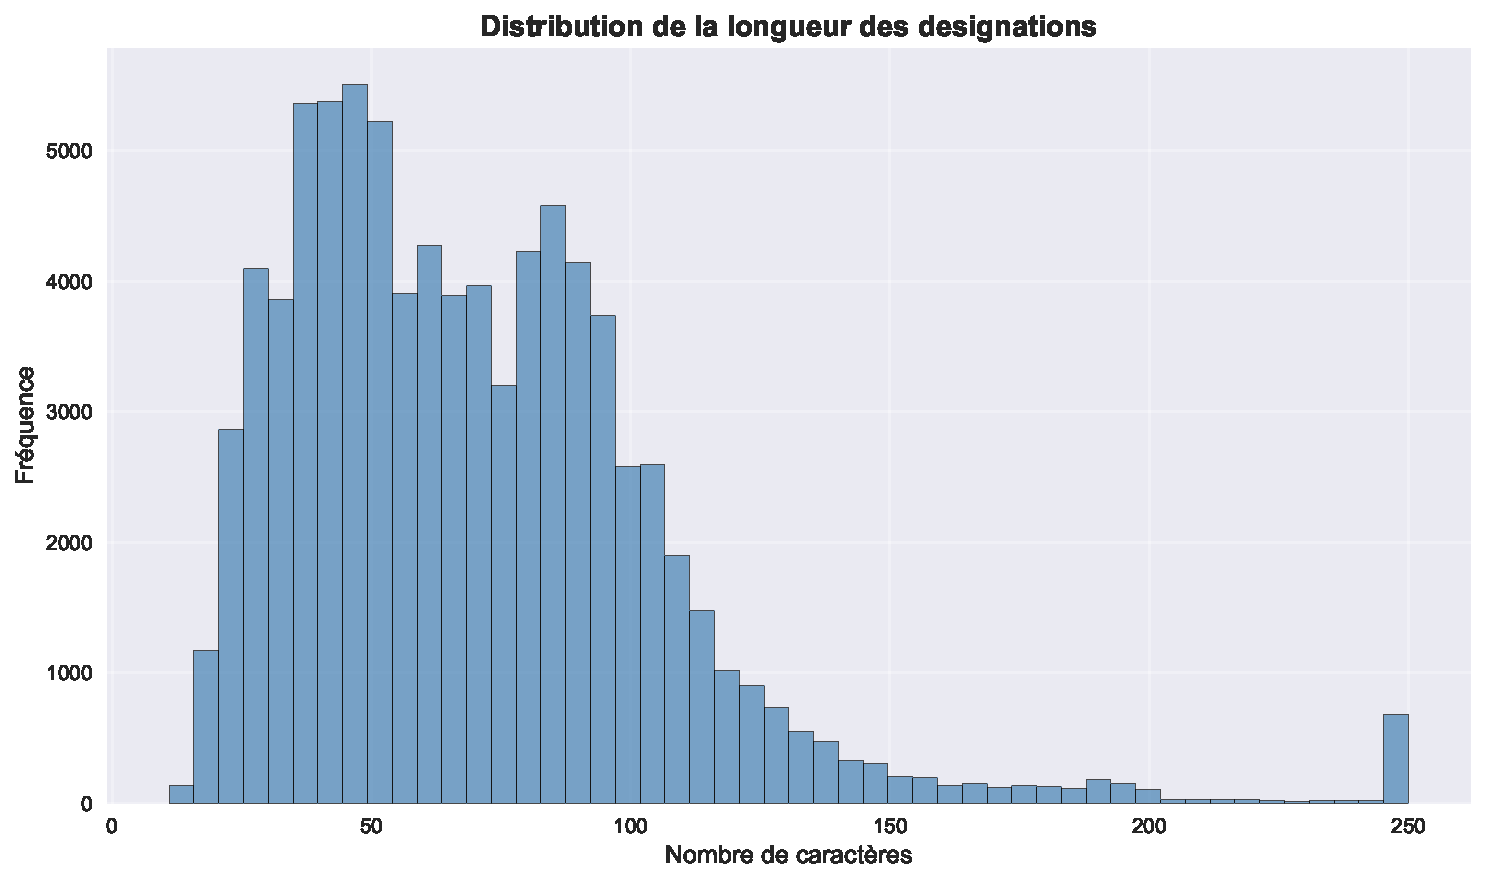
\includegraphics[width=0.85\textwidth]{figures/01_distribution_longueur_designation.pdf}
    \caption{Distribution de la longueur des designations (en caractères)}
    \label{fig:distribution_longueur_designation}
\end{figure}

\begin{figure}[H]
    \centering
    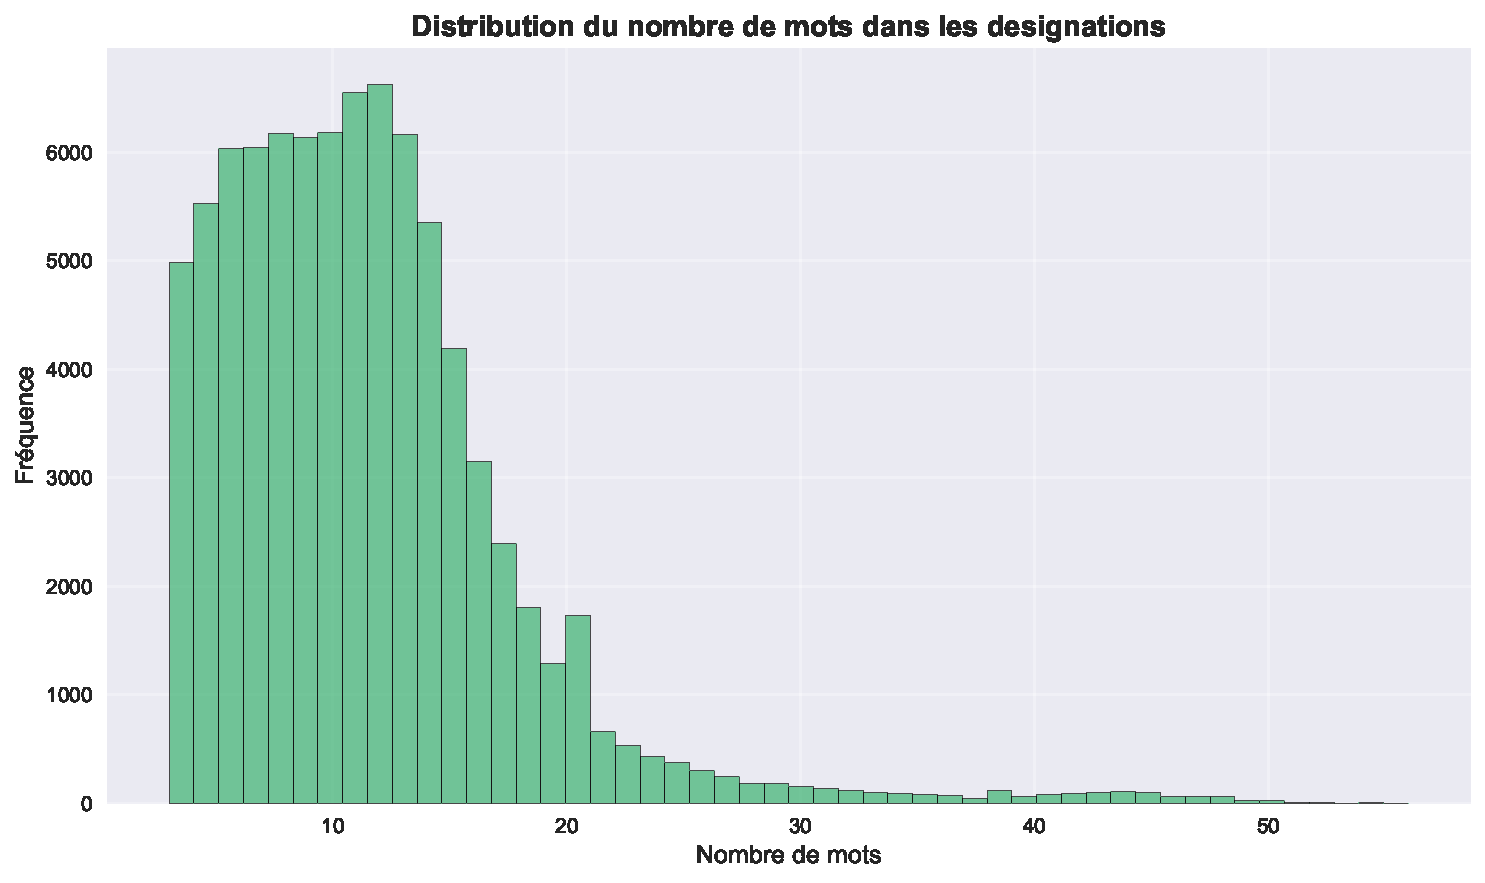
\includegraphics[width=0.85\textwidth]{figures/03_distribution_mots_designation.pdf}
    \caption{Distribution du nombre de mots dans les designations}
    \label{fig:distribution_mots_designation}
\end{figure}

\textbf{Distribution :} Les figures~\ref{fig:distribution_longueur_designation} et~\ref{fig:distribution_mots_designation} montrent une distribution avec une asymétrie légère vers la droite (plus de designations courtes). Les designations sont généralement concises et informatives, avec un pic autour de 40-50 caractères (soit environ 6-8 mots) et un second pic autour de 80-90 caractères (soit environ 12-15 mots).

\subsubsection{Description}

\begin{table}[H]
\centering
\begin{tabular}{@{}lr@{}}
\toprule
\textbf{Statistique} & \textbf{Valeur} \\
\midrule
Longueur moyenne (non vides) & 525.61 caractères \\
Longueur médiane (non vides) & 231.00 caractères \\
Écart-type (non vides) & ~800 caractères \\
Minimum & 1 caractère \\
Maximum & 12~451 caractères \\
Nombre de mots moyen (non vides) & 80.17 mots \\
Descriptions vides ou NaN & 59~600 (70,19~\%) \\
\bottomrule
\end{tabular}
\caption{Statistiques descriptives des descriptions}
\label{tab:stats_description}
\end{table}

\begin{figure}[H]
    \centering
    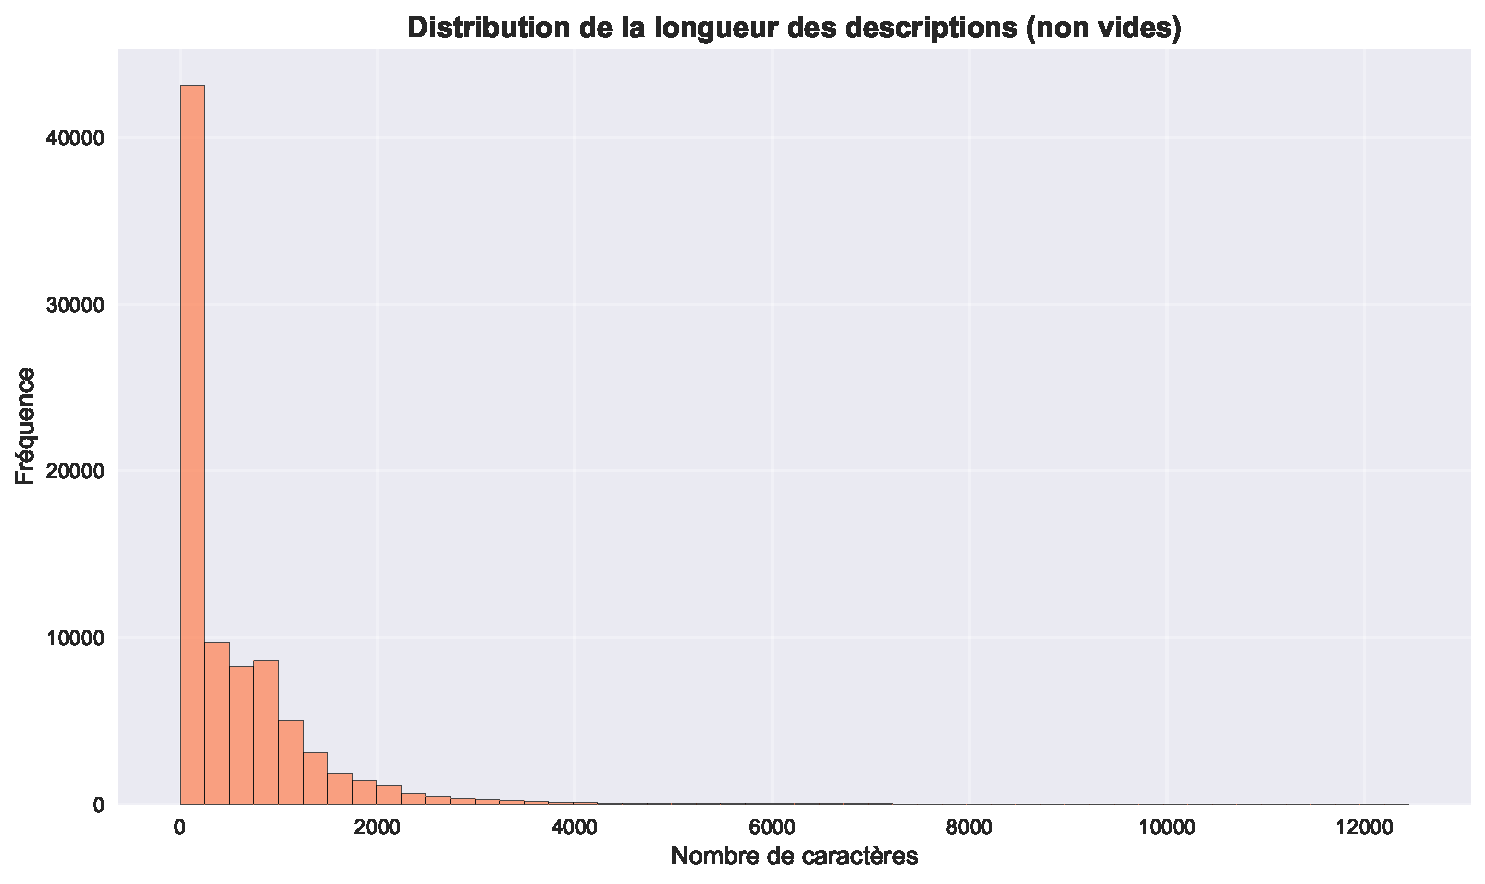
\includegraphics[width=0.85\textwidth]{figures/02_distribution_longueur_description.pdf}
    \caption{Distribution de la longueur des descriptions non vides (en caractères)}
    \label{fig:distribution_longueur_description}
\end{figure}

\begin{figure}[H]
    \centering
    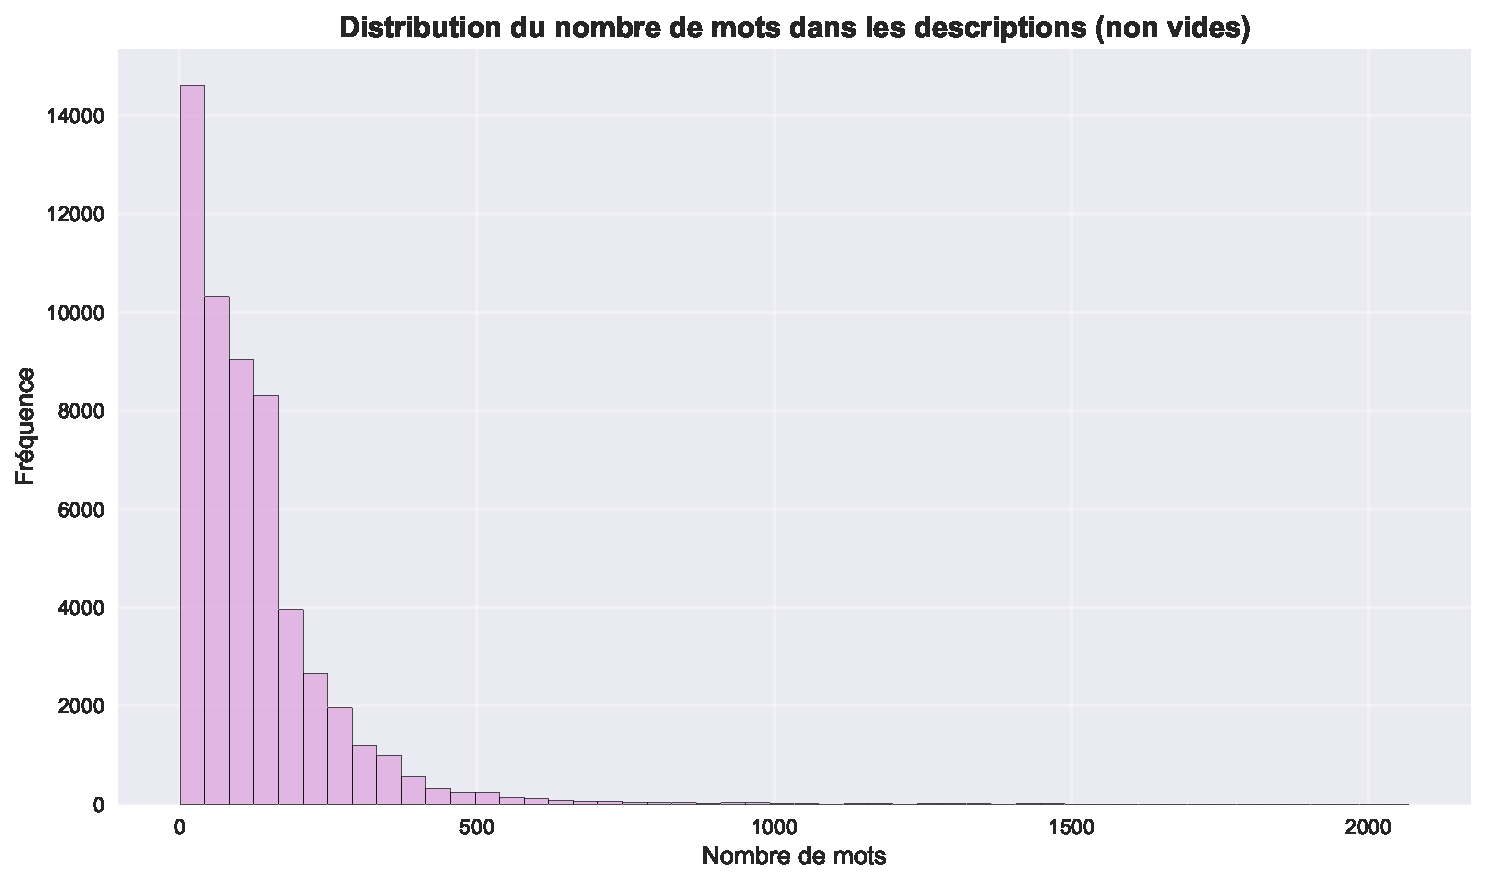
\includegraphics[width=0.85\textwidth]{figures/04_distribution_mots_description.pdf}
    \caption{Distribution du nombre de mots dans les descriptions non vides}
    \label{fig:distribution_mots_description}
\end{figure}

\textbf{Distribution :} Les figures~\ref{fig:distribution_longueur_description} et~\ref{fig:distribution_mots_description} montrent une forte asymétrie (distribution très étalée, avec quelques descriptions très longues). La majorité des descriptions non vides se concentrent entre 50 et 500 caractères (soit environ 8 à 80 mots), mais il existe des valeurs extrêmes allant jusqu'à plus de 12~000 caractères. 

\textbf{Implications :}
\begin{itemize}
    \item Traitement différencié nécessaire pour les descriptions vides vs non vides
    \item Possible nécessité de tronquer les descriptions très longues
    \item La description n'est pas toujours disponible, donc la designation est cruciale
\end{itemize}

Ces observations préliminaires nous amènent à analyser plus en détail la distribution statistique des catégories.

\section{Analyse statistique descriptive}

\subsection{Distribution des catégories}

Le dataset contient \textbf{27 catégories différentes} de produits, identifiées par des codes numériques allant de 10 à 2583.

\subsubsection{Top 10 catégories les plus fréquentes}

\begin{table}[H]
\centering
\begin{tabular}{@{}lrrr@{}}
\toprule
\textbf{Rang} & \textbf{Catégorie} & \textbf{Nombre} & \textbf{Pourcentage} \\
\midrule
1 & 2583 & 10~209 & 12,02~\% \\
2 & 1560 & 5~073 & 5,98~\% \\
3 & 1300 & 5~045 & 5,94~\% \\
4 & 1280 & 4~870 & 5,74~\% \\
5 & 2403 & 4~774 & 5,62~\% \\
6 & 2280 & 4~760 & 5,61~\% \\
7 & 2060 & 4~993 & 5,88~\% \\
8 & 1920 & 4~303 & 5,07~\% \\
9 & 1320 & 3~241 & 3,82~\% \\
10 & 1160 & 3~953 & 4,66~\% \\
\midrule
\textbf{Total Top 10} & & 50~221 & \textbf{59,22~\%} \\
\bottomrule
\end{tabular}
\caption{Top 10 catégories les plus fréquentes}
\label{tab:top10_categories}
\end{table}

\begin{figure}[H]
    \centering
    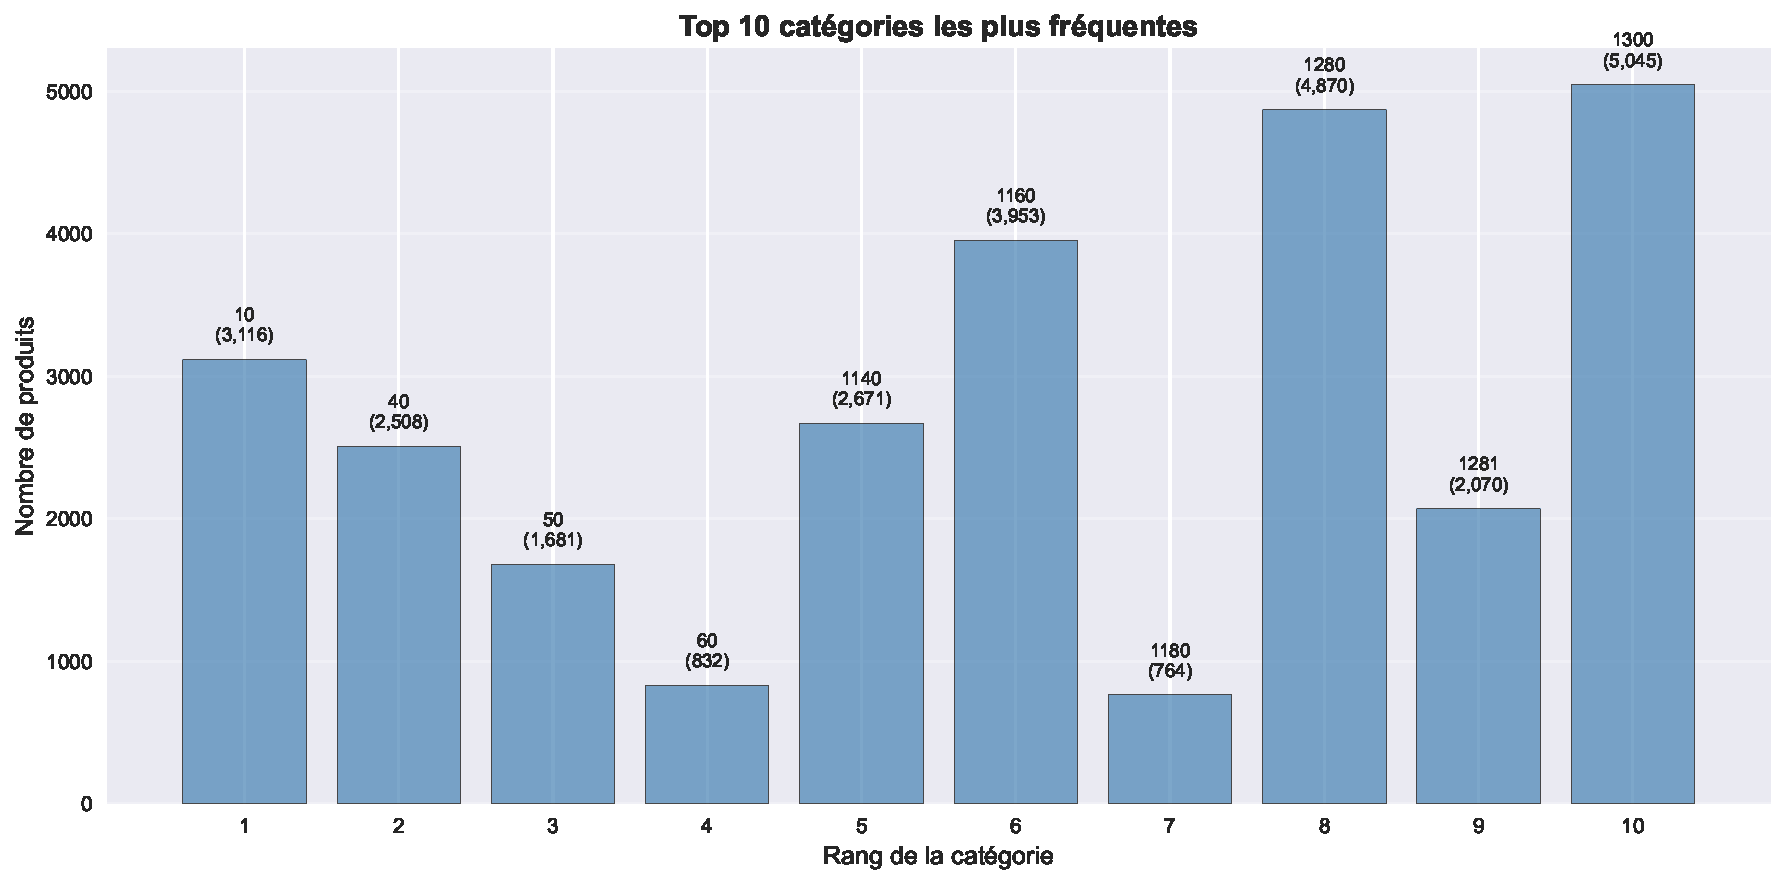
\includegraphics[width=0.85\textwidth]{figures/05_top10_categories.pdf}
    \caption{Top 10 catégories les plus fréquentes (nombre de produits par catégorie)}
    \label{fig:top10_categories}
\end{figure}

La figure~\ref{fig:top10_categories} présente les 10 catégories les plus fréquentes du dataset. Les catégories affichées correspondent à celles du tableau~\ref{tab:top10_categories} : 2583, 1560, 1300, 1280, 2403, 2280, 2060, 1920, 1320, 1160. On observe une distribution décroissante avec la catégorie 2583 en tête (12,02~\% des données), suivie par les catégories 1560 et 1300 (environ 6~\% chacune).

\subsection{Analyse du déséquilibre des classes}
\label{sec:desequilibre}

Le dataset présente un \textbf{déséquilibre modéré à important} :

\begin{itemize}
    \item \textbf{Catégorie la plus fréquente} : 12,02~\% des données (catégorie 2583)
    \item \textbf{Catégorie la moins fréquente} : 0,90~\% des données (catégorie 1180 avec 764 produits)
    \item \textbf{Ratio max/min} : 13,4
\end{itemize}

\subsubsection{Distribution cumulative}

\begin{figure}[H]
    \centering
    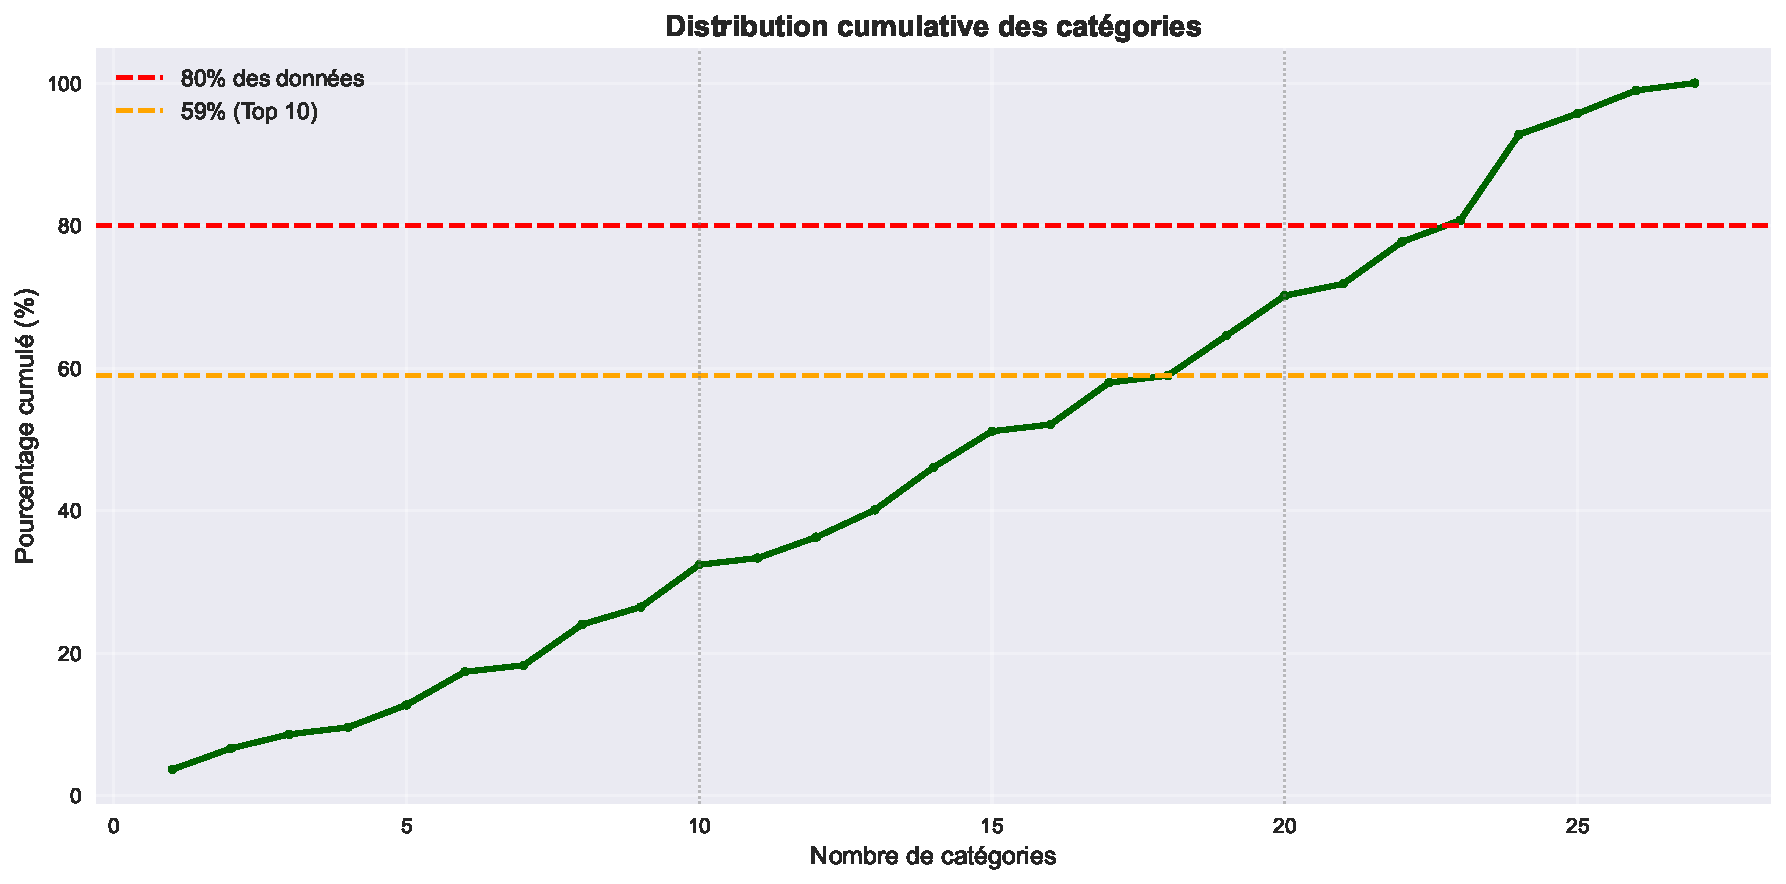
\includegraphics[width=0.85\textwidth]{figures/06_distribution_cumulative_categories.pdf}
    \caption{Distribution cumulative des catégories (pourcentage cumulé en fonction du nombre de catégories)}
    \label{fig:distribution_cumulative}
\end{figure}

La figure~\ref{fig:distribution_cumulative} illustre la distribution cumulative des catégories. On observe que :

\begin{itemize}
    \item Les \textbf{10 premières catégories} représentent environ \textbf{59\%} des données
    \item Les \textbf{20 premières catégories} représentent environ \textbf{80\%} des données
    \item Les \textbf{27 catégories} sont toutes représentées
\end{itemize}

\subsubsection{Implications pour la modélisation}

Ce déséquilibre nécessitera l'utilisation de techniques spécifiques :

\begin{enumerate}
    \item \textbf{Pondération des classes} : Donner plus de poids aux classes minoritaires
    \item \textbf{Métriques adaptées} : Utiliser F1-score macro/micro plutôt que accuracy
    \item \textbf{Techniques de rééchantillonnage} : Si nécessaire (SMOTE, undersampling, etc.)
    \item \textbf{Stratification} : Dans la validation croisée pour maintenir les proportions
\end{enumerate}

Fort de cette compréhension de la distribution des données, nous pouvons maintenant approfondir l'analyse à travers des visualisations détaillées.

\section{Visualisations et analyses approfondies}

\subsection{Distribution des longueurs de textes}

\subsubsection{Histogrammes des longueurs}

Cette visualisation présente quatre histogrammes :

\begin{enumerate}
    \item \textbf{Distribution de la longueur des designations} : Histogramme montrant le nombre de caractères dans les designations
    \item \textbf{Distribution de la longueur des descriptions (non vides)} : Histogramme pour les descriptions avec du contenu
    \item \textbf{Distribution du nombre de mots dans les designations} : Granularité plus fine avec le comptage de mots
    \item \textbf{Distribution du nombre de mots dans les descriptions (non vides)} : Nombre de mots pour les descriptions
\end{enumerate}

\begin{figure}[H]
    \centering
    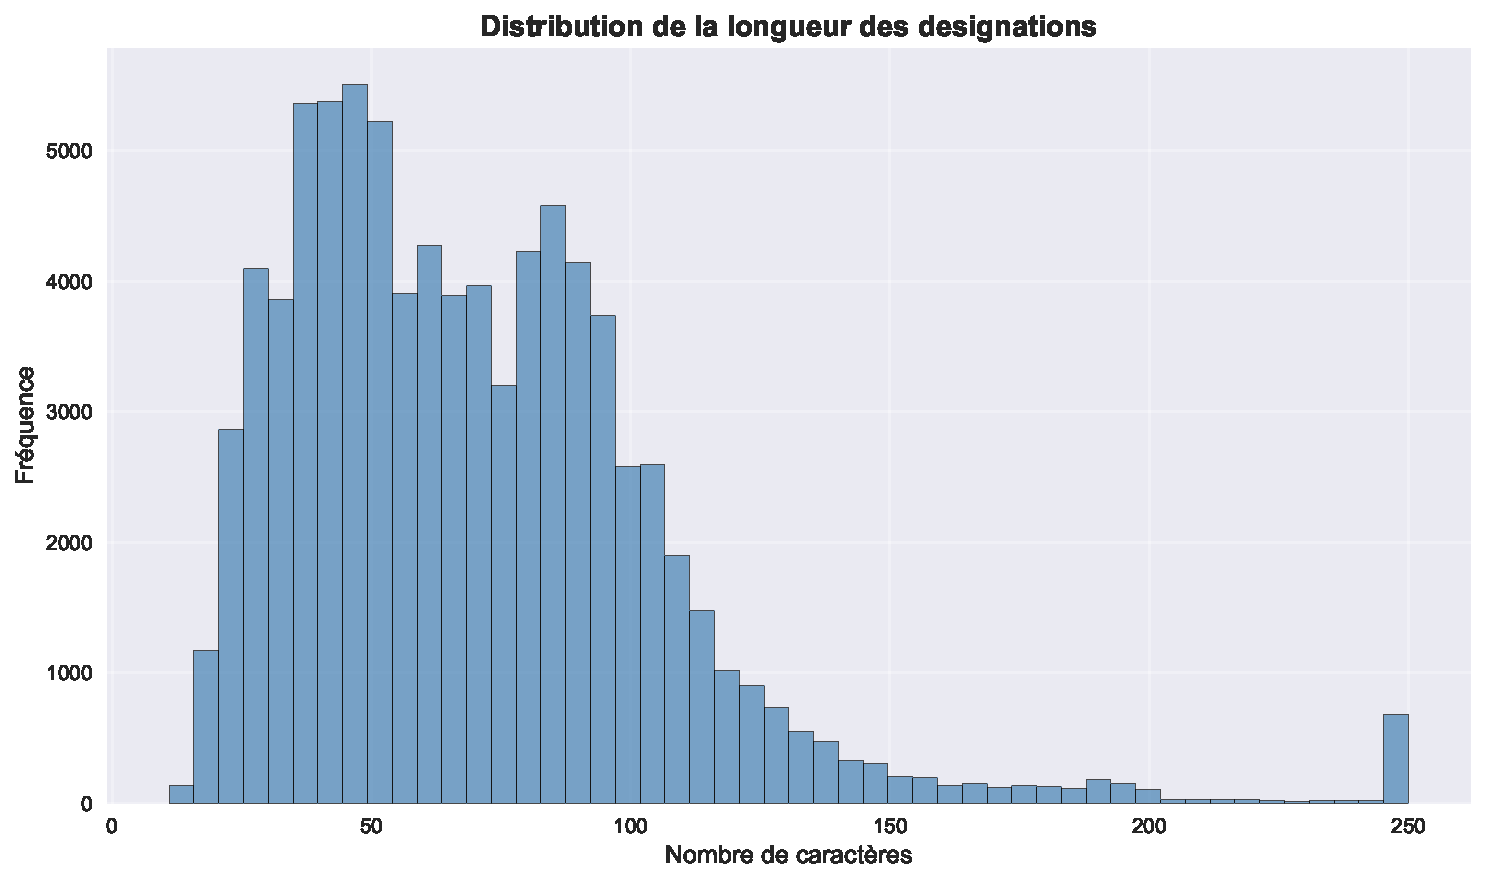
\includegraphics[width=0.85\textwidth]{figures/01_distribution_longueur_designation.pdf}
    \caption{Distribution de la longueur des designations (en caractères)}
    \label{fig:hist_longueur_designation}
\end{figure}

\begin{figure}[H]
    \centering
    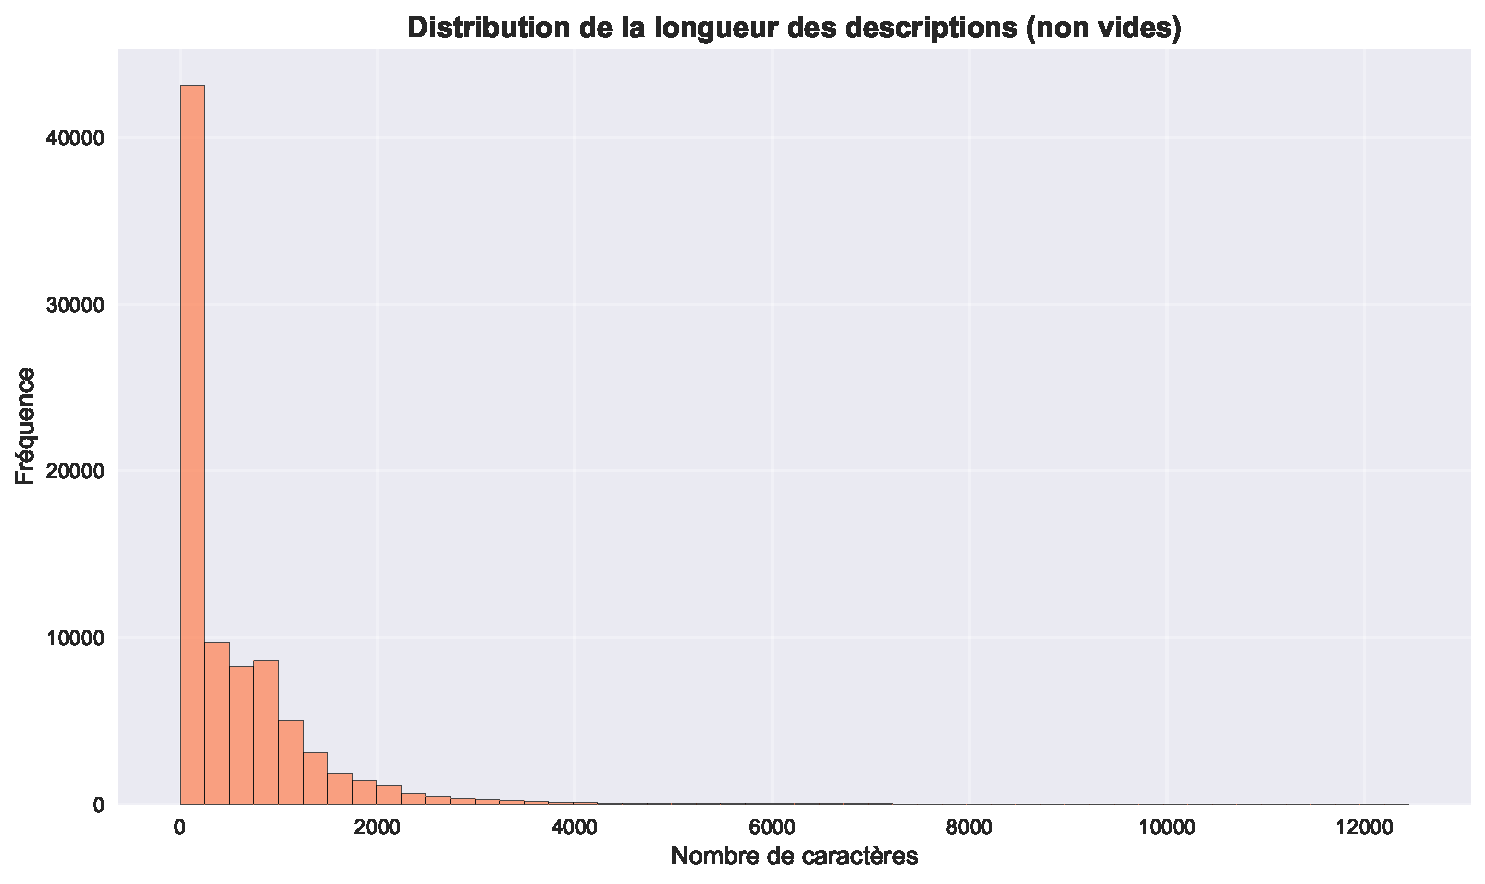
\includegraphics[width=0.85\textwidth]{figures/02_distribution_longueur_description.pdf}
    \caption{Distribution de la longueur des descriptions non vides (en caractères)}
    \label{fig:hist_longueur_description}
\end{figure}

\begin{figure}[H]
    \centering
    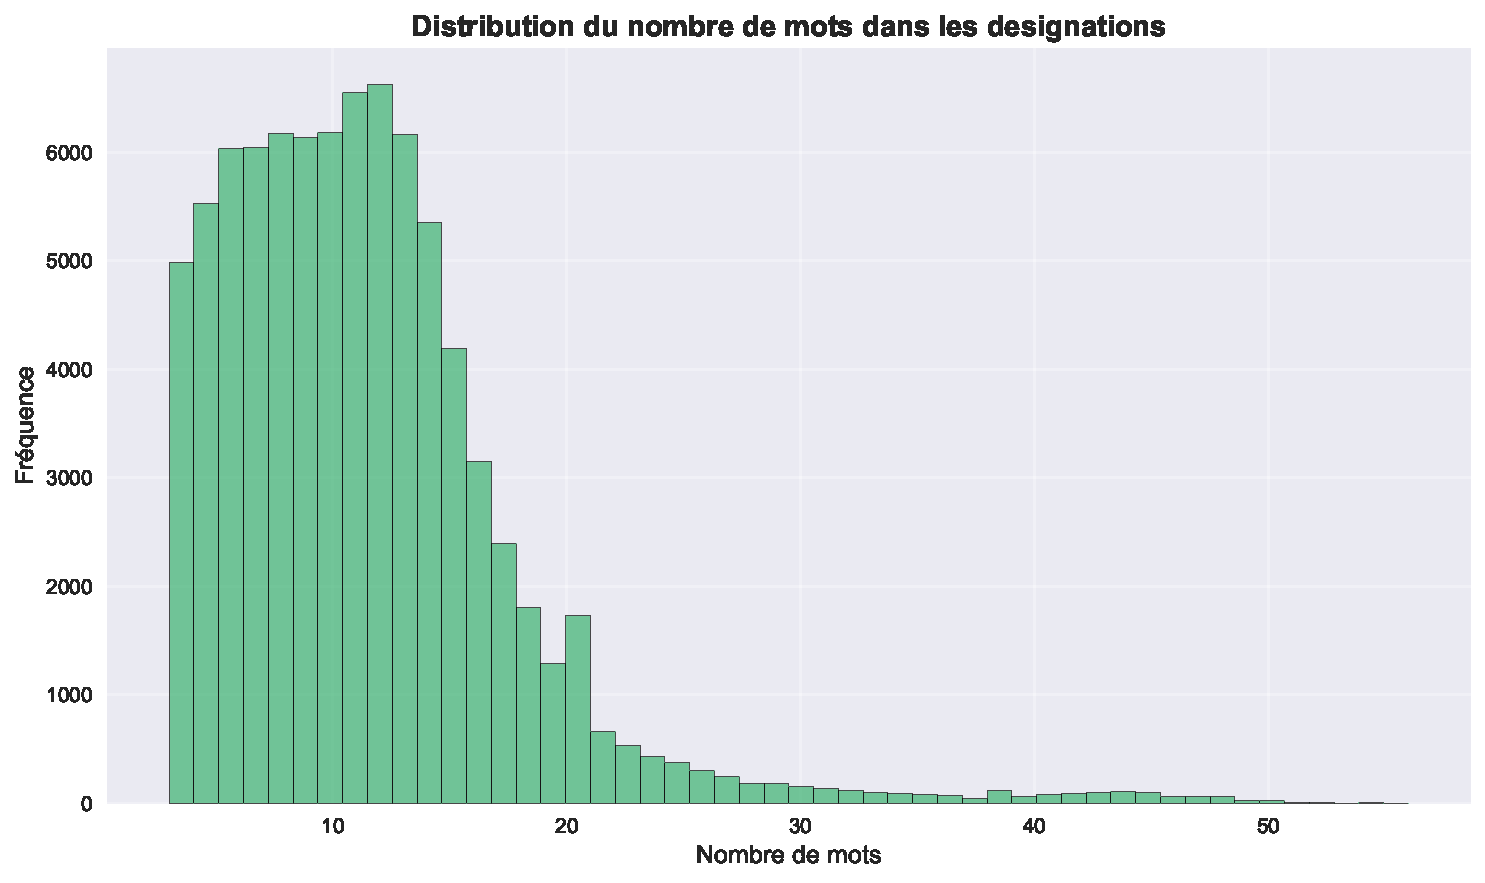
\includegraphics[width=0.85\textwidth]{figures/03_distribution_mots_designation.pdf}
    \caption{Distribution du nombre de mots dans les designations}
    \label{fig:hist_mots_designation}
\end{figure}

\begin{figure}[H]
    \centering
    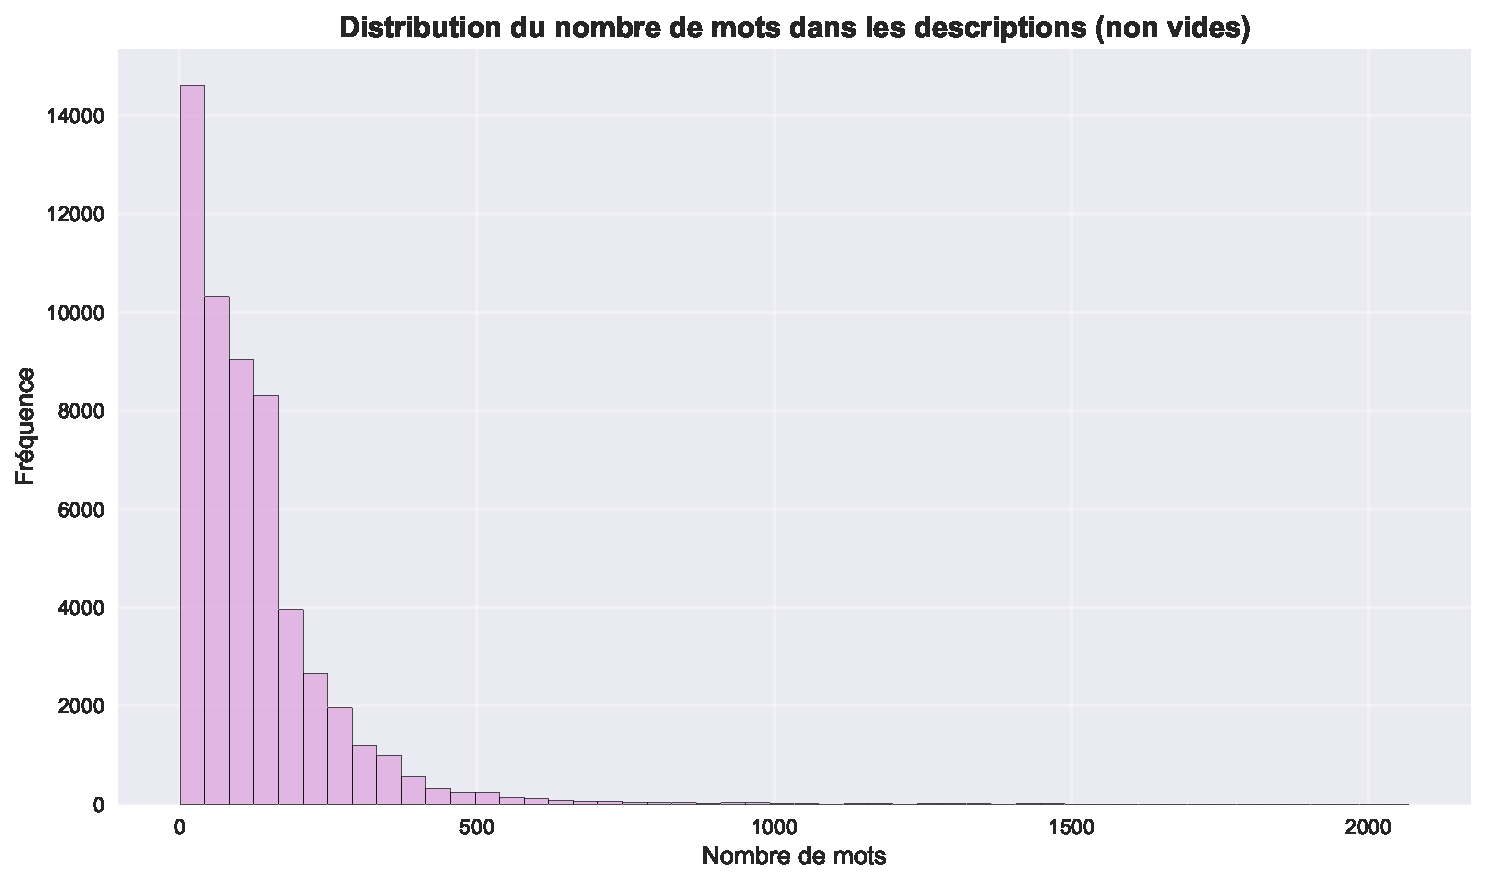
\includegraphics[width=0.85\textwidth]{figures/04_distribution_mots_description.pdf}
    \caption{Distribution du nombre de mots dans les descriptions non vides}
    \label{fig:hist_mots_description}
\end{figure}

\textbf{Interprétation :}
\begin{itemize}
    \item Les figures~\ref{fig:hist_longueur_designation} et~\ref{fig:hist_mots_designation} montrent que les designations suivent une distribution relativement normale avec une légère asymétrie positive
    \item Pic autour de 50-70 caractères (soit environ 8-12 mots) pour les designations
    \item Les figures~\ref{fig:hist_longueur_description} et~\ref{fig:hist_mots_description} montrent que les descriptions présentent une forte asymétrie avec quelques valeurs extrêmes très élevées
    \item La plupart des descriptions non vides sont courtes ($<$ 500 caractères, soit environ $<$ 80 mots)
    \item Présence de quelques descriptions très longues ($>$ 5000 caractères) qui pourraient nécessiter un traitement spécial
\end{itemize}

\subsection{Distribution des catégories}

\subsubsection{Distribution des 30 catégories les plus fréquentes}

\begin{figure}[H]
    \centering
    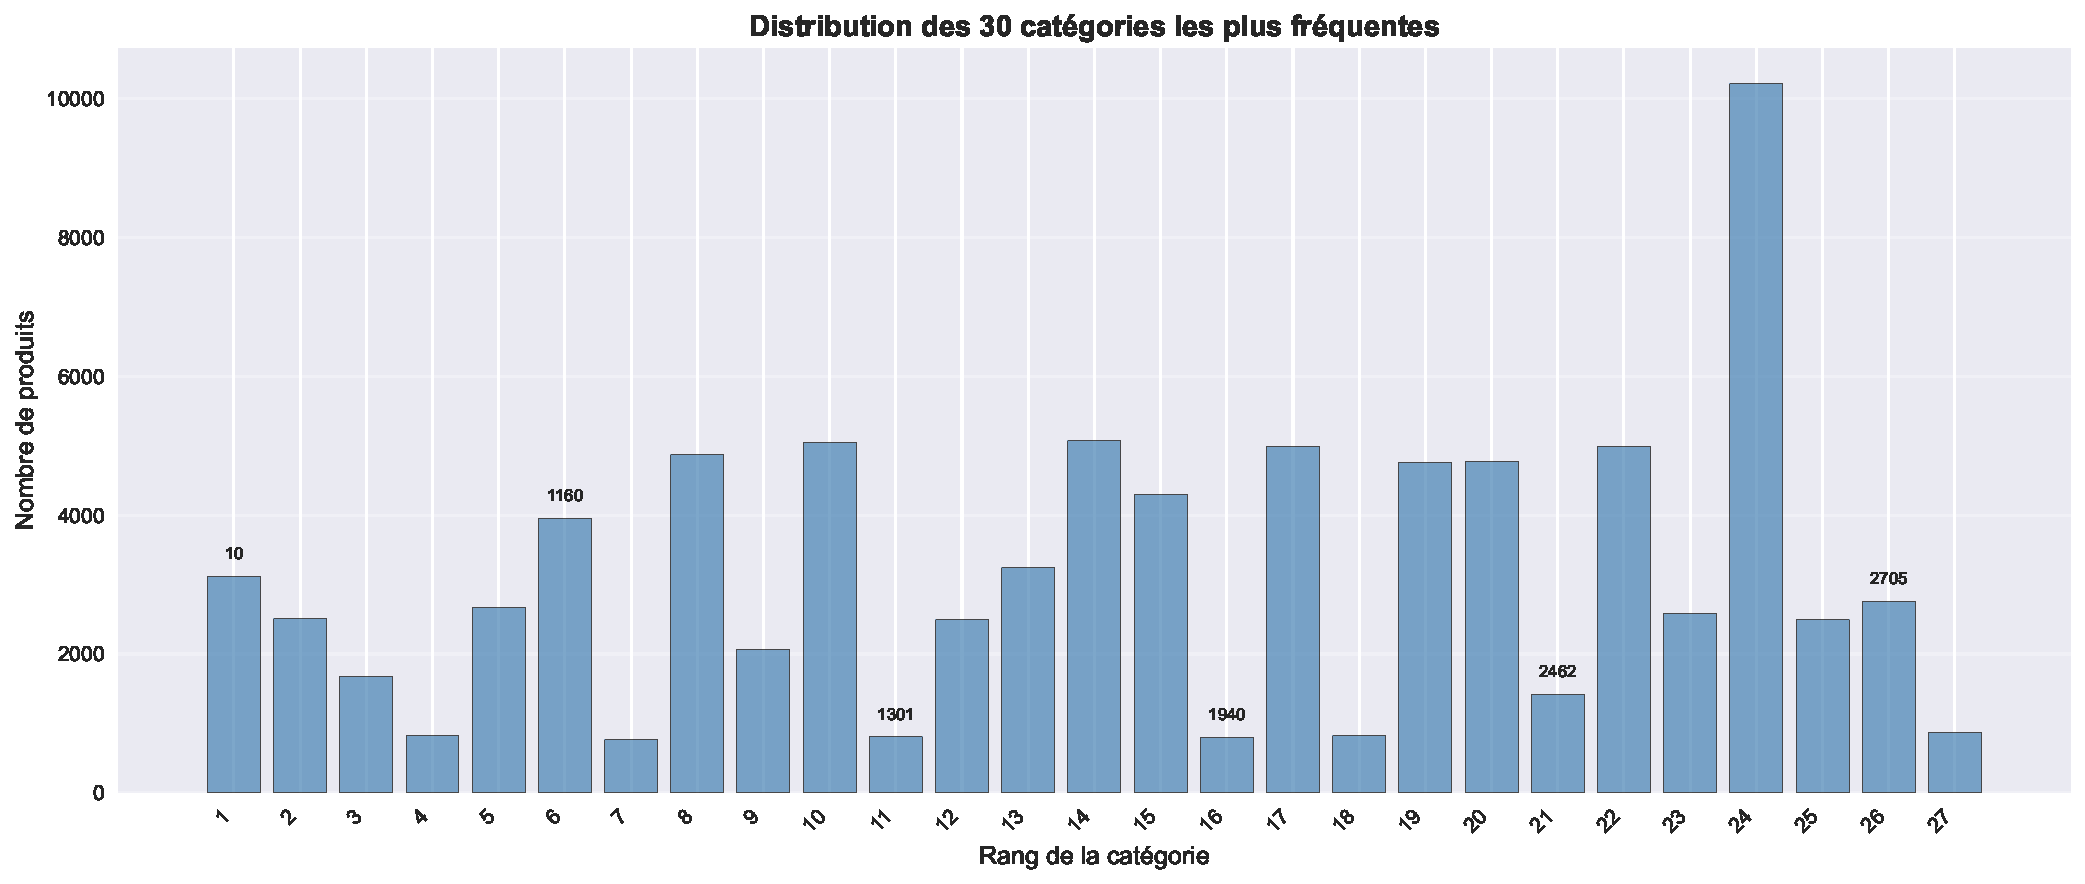
\includegraphics[width=0.9\textwidth]{figures/07_distribution_30_categories.pdf}
    \caption{Distribution des 30 catégories les plus fréquentes (nombre de produits par catégorie)}
    \label{fig:distribution_30_categories}
\end{figure}

La figure~\ref{fig:distribution_30_categories} présente un graphique en barres montrant la distribution des catégories.

\textbf{Observations :}
\begin{itemize}
    \item Les catégories les plus fréquentes dominent visuellement
    \item Déclin progressif vers les catégories moins fréquentes
    \item Pas de catégorie vraiment dominante (> 15\% des données)
    \item Distribution relativement équilibrée entre les catégories principales
\end{itemize}

\subsubsection{Distribution cumulative}

La figure~\ref{fig:distribution_cumulative} (présentée dans la section~\ref{sec:desequilibre}) montre le pourcentage cumulé des données par nombre de catégories.

\textbf{Observations :}
\begin{itemize}
    \item Les 10 premières catégories représentent environ 59\% des données
    \item Les 20 premières catégories représentent environ 80\% des données (ligne de référence à 80\%)
    \item Convergence progressive vers 100\% avec les 27 catégories
\end{itemize}

\textbf{Interprétation :}
Cette distribution cumulative montre que la majorité des données est concentrée dans un nombre relativement restreint de catégories, ce qui peut faciliter la classification des catégories principales mais rendre plus difficile la classification des catégories minoritaires.

\subsection{Analyse par catégorie}

\subsubsection{Boxplots de longueur par catégorie (Top 10)}

Deux boxplots séparés :
\begin{enumerate}
    \item \textbf{Distribution de la longueur des designations par catégorie} : Variation de la longueur des designations selon la catégorie
    \item \textbf{Distribution de la longueur des descriptions par catégorie} : Variation de la longueur des descriptions selon la catégorie
\end{enumerate}

\begin{figure}[H]
    \centering
    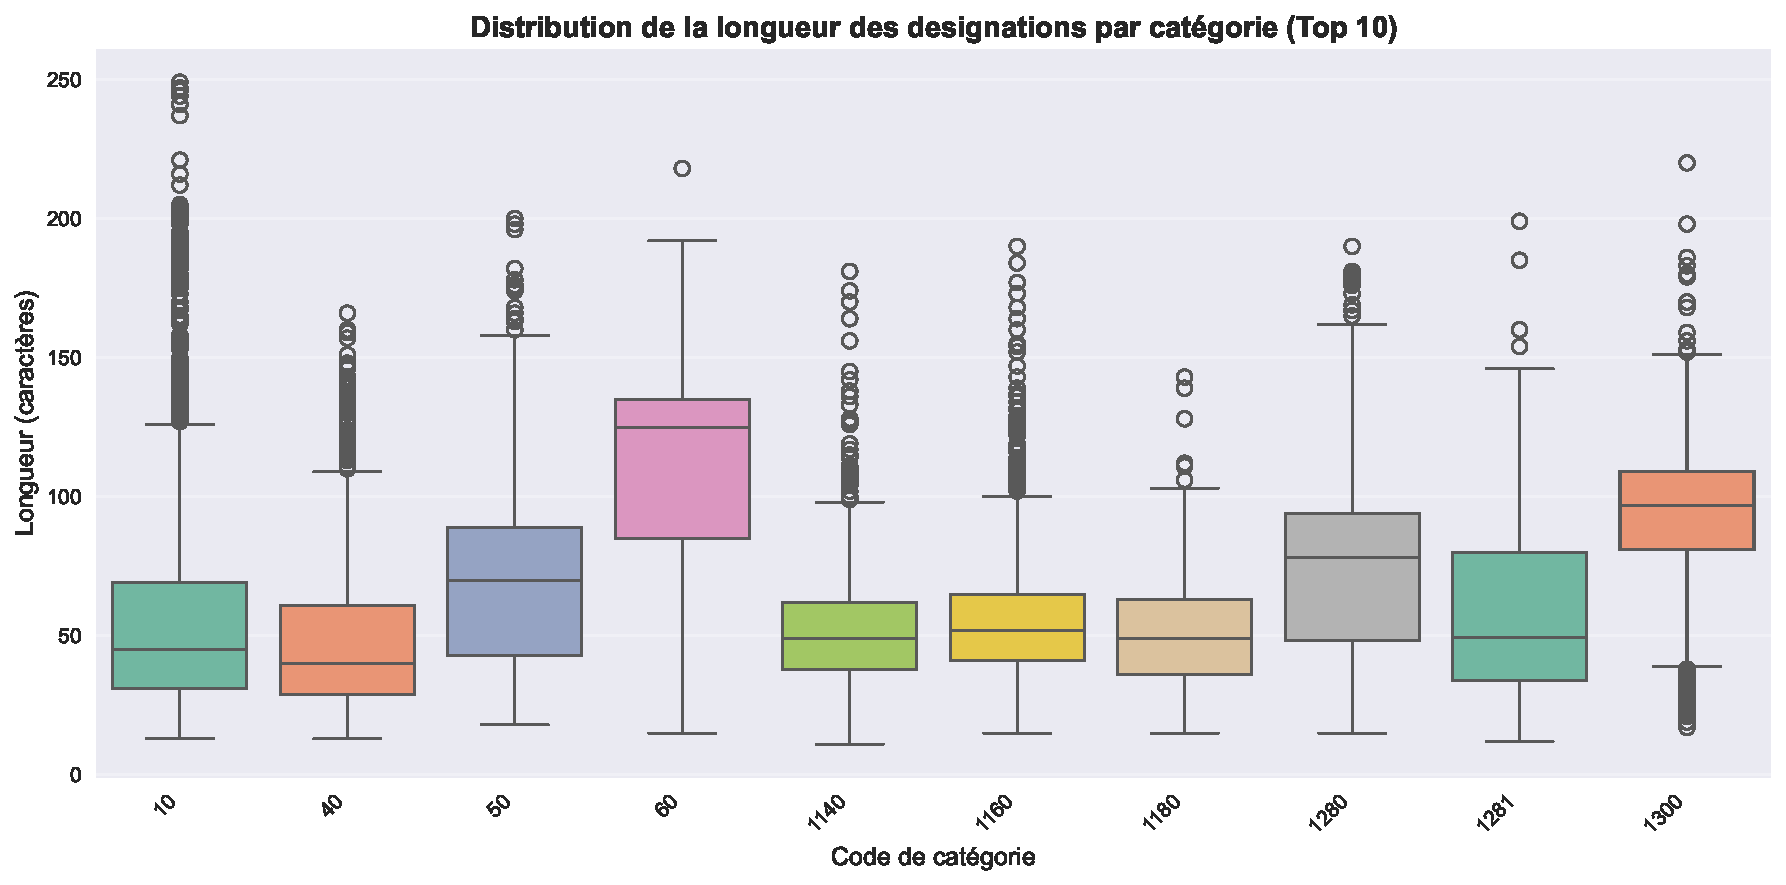
\includegraphics[width=0.9\textwidth]{figures/08_boxplot_designation_categories.pdf}
    \caption{Distribution de la longueur des designations par catégorie (Top 10)}
    \label{fig:boxplot_designation_categories}
\end{figure}

\begin{figure}[H]
    \centering
    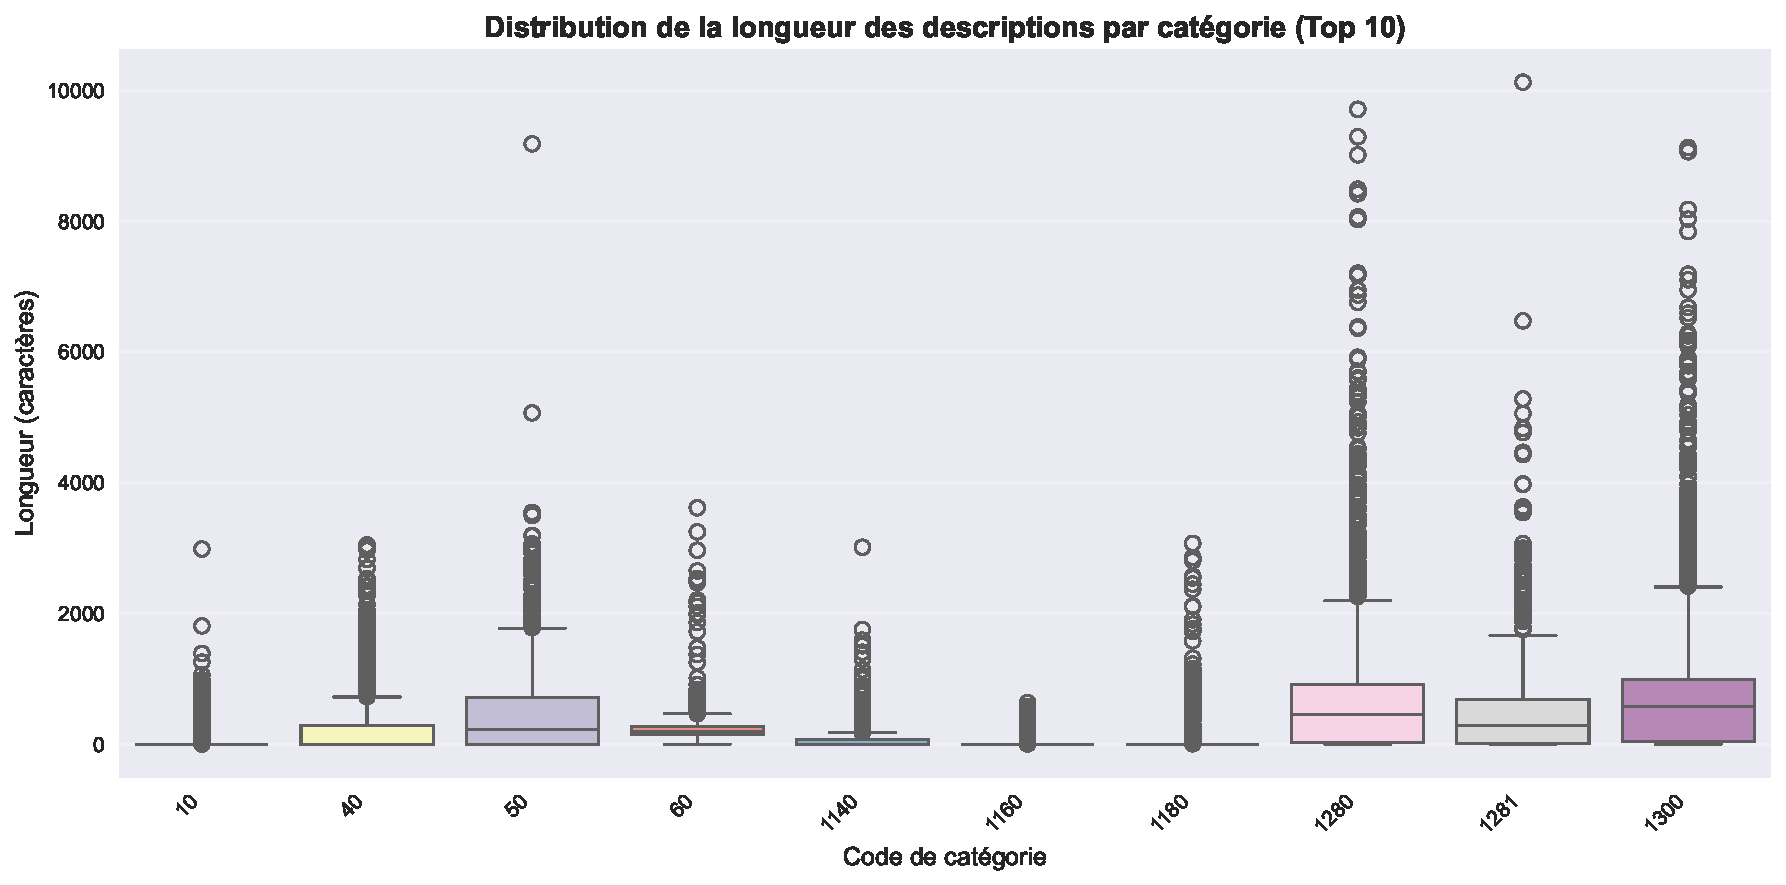
\includegraphics[width=0.9\textwidth]{figures/09_boxplot_description_categories.pdf}
    \caption{Distribution de la longueur des descriptions par catégorie (Top 10)}
    \label{fig:boxplot_description_categories}
\end{figure}

\textbf{Observations :}
Les figures~\ref{fig:boxplot_designation_categories} et~\ref{fig:boxplot_description_categories} montrent :
\begin{itemize}
    \item Variation significative de la longueur moyenne selon la catégorie
    \item Certaines catégories ont des designations plus descriptives que d'autres
    \item Cette différence peut être une feature discriminante importante
    \item Présence de valeurs aberrantes dans certaines catégories (points en dehors des moustaches)
    \item Les médianes varient considérablement entre catégories
\end{itemize}

\textbf{Interprétation :}
Les différences de longueur entre catégories suggèrent que certaines catégories nécessitent plus d'informations pour être décrites (par exemple, produits techniques vs produits simples). Ces patterns peuvent être exploités par le modèle de classification.

\subsection{Présence de description par catégorie}

\subsubsection{Taux de présence des descriptions}

\begin{figure}[H]
    \centering
    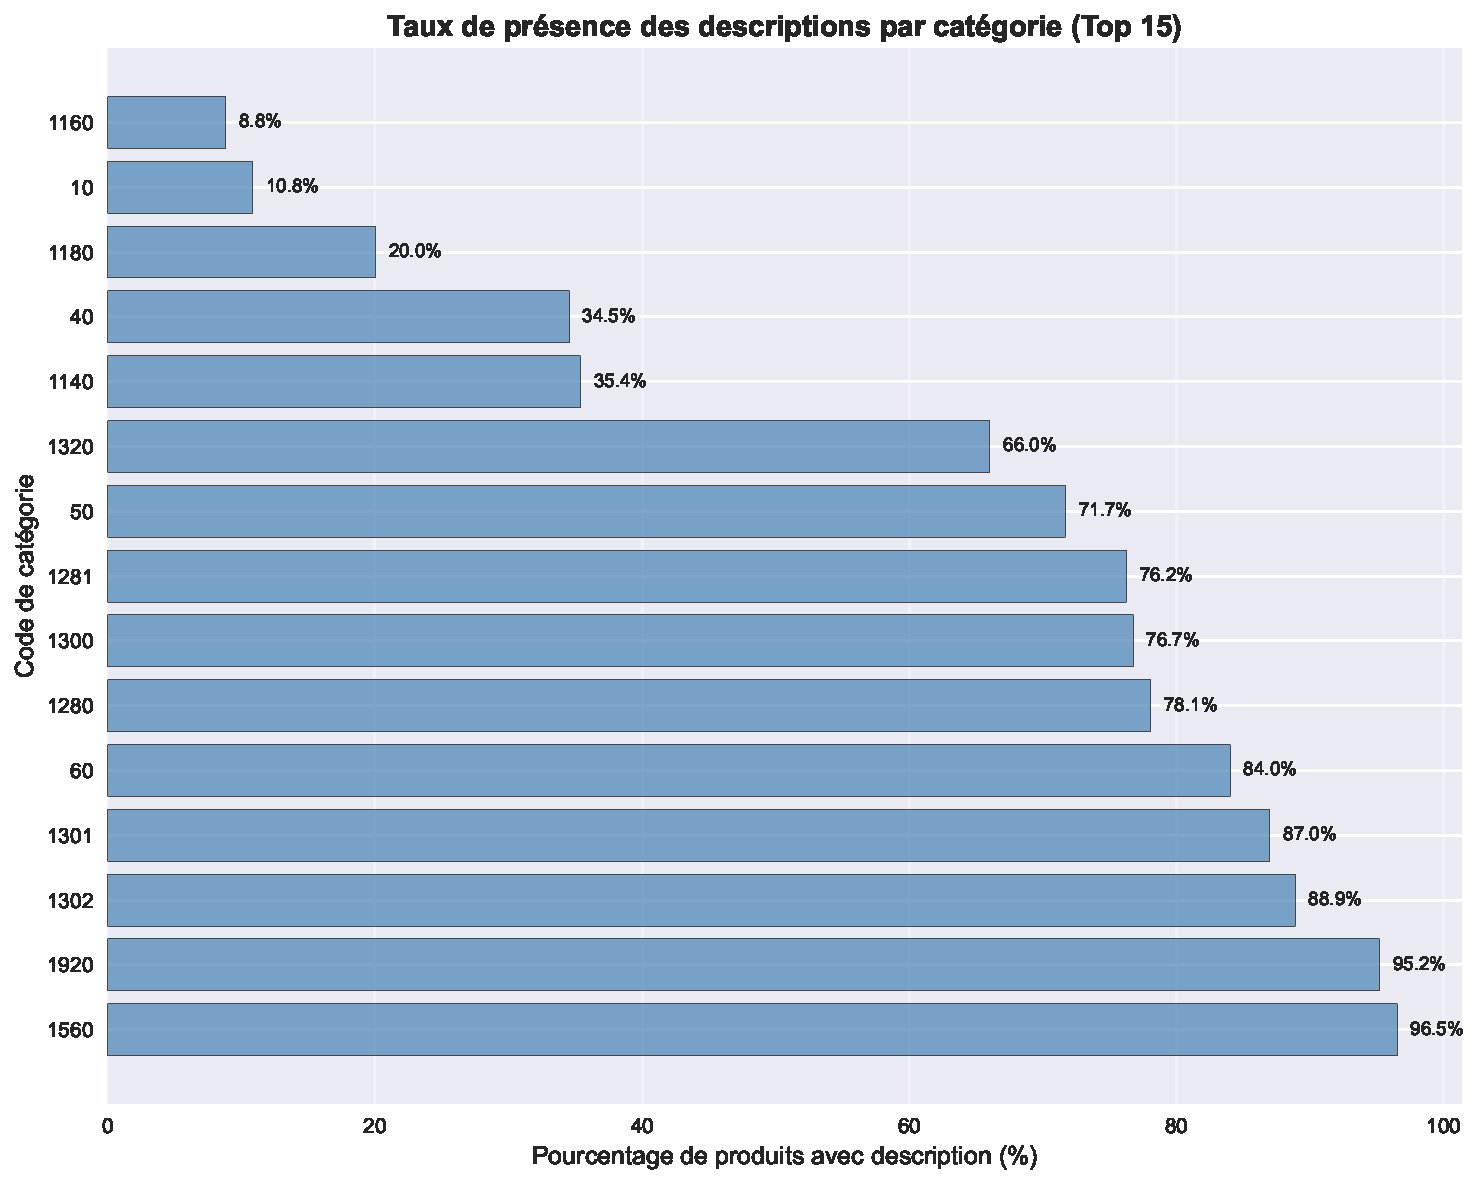
\includegraphics[width=0.85\textwidth]{figures/10_taux_presence_descriptions.pdf}
    \caption{Taux de présence des descriptions par catégorie (Top 15 catégories)}
    \label{fig:taux_presence_descriptions}
\end{figure}

La figure~\ref{fig:taux_presence_descriptions} présente un graphique en barres horizontales montrant le pourcentage de produits ayant une description pour les 15 catégories principales.

\textbf{Observations :}
\begin{itemize}
    \item Le taux de présence de description varie considérablement selon la catégorie
    \item Certaines catégories ont plus souvent des descriptions que d'autres
    \item Variation de ~20\% à ~50\% selon les catégories
    \item Peut indiquer des différences dans les pratiques de saisie selon la catégorie
\end{itemize}

\textbf{Interprétation :}
Cette variation suggère que certaines catégories bénéficient plus que d'autres de l'information supplémentaire fournie par les descriptions. Le modèle devra être capable de gérer efficacement les cas où la description est absente.

\subsubsection{Impact de la présence de description}

\begin{figure}[H]
    \centering
    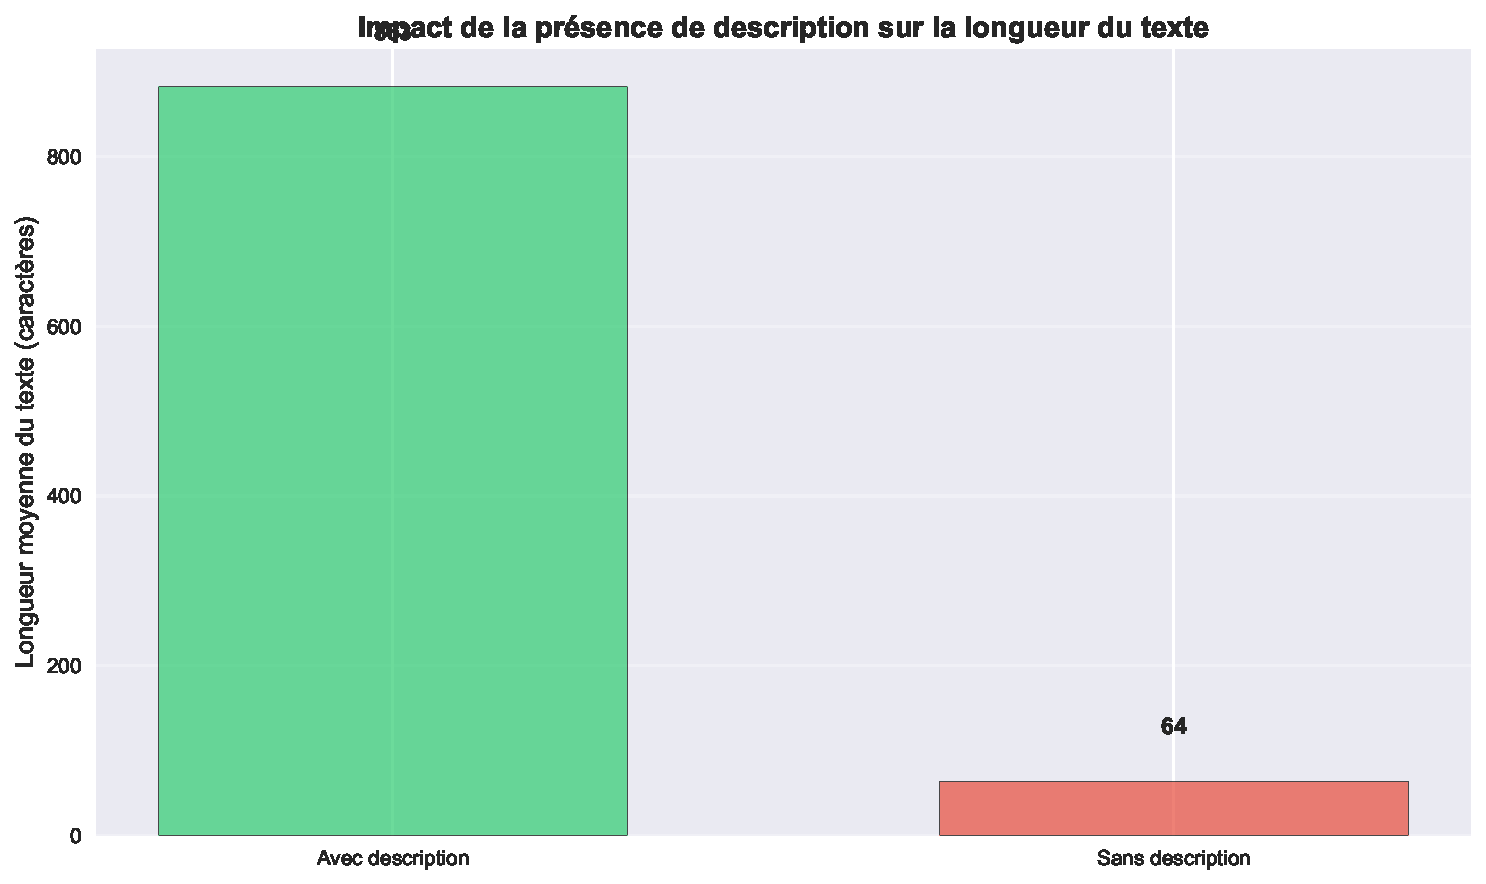
\includegraphics[width=0.75\textwidth]{figures/11_impact_presence_description.pdf}
    \caption{Impact de la présence de description sur la longueur moyenne du texte}
    \label{fig:impact_presence_description}
\end{figure}

La figure~\ref{fig:impact_presence_description} présente un graphique en barres comparant la longueur moyenne du texte avec et sans description.

\textbf{Observations :}
\begin{itemize}
    \item Les produits avec description ont une longueur totale de texte significativement plus élevée
    \item Différence marquée entre les deux catégories (avec/ sans description)
    \item Impact direct sur la quantité d'information disponible pour la classification
\end{itemize}

\textbf{Interprétation :}
La présence d'une description apporte une information textuelle supplémentaire substantielle. Cependant, le modèle doit être robuste car 70\% des produits n'ont pas de description.

\subsection{Analyse de la langue}

\subsubsection{Distribution des langues}

Deux visualisations :
\begin{enumerate}
    \item \textbf{Camembert} : Distribution globale des langues dans un échantillon
    \item \textbf{Barres empilées} : Distribution des langues par catégorie (Top 5)
\end{enumerate}

\begin{figure}[H]
    \centering
    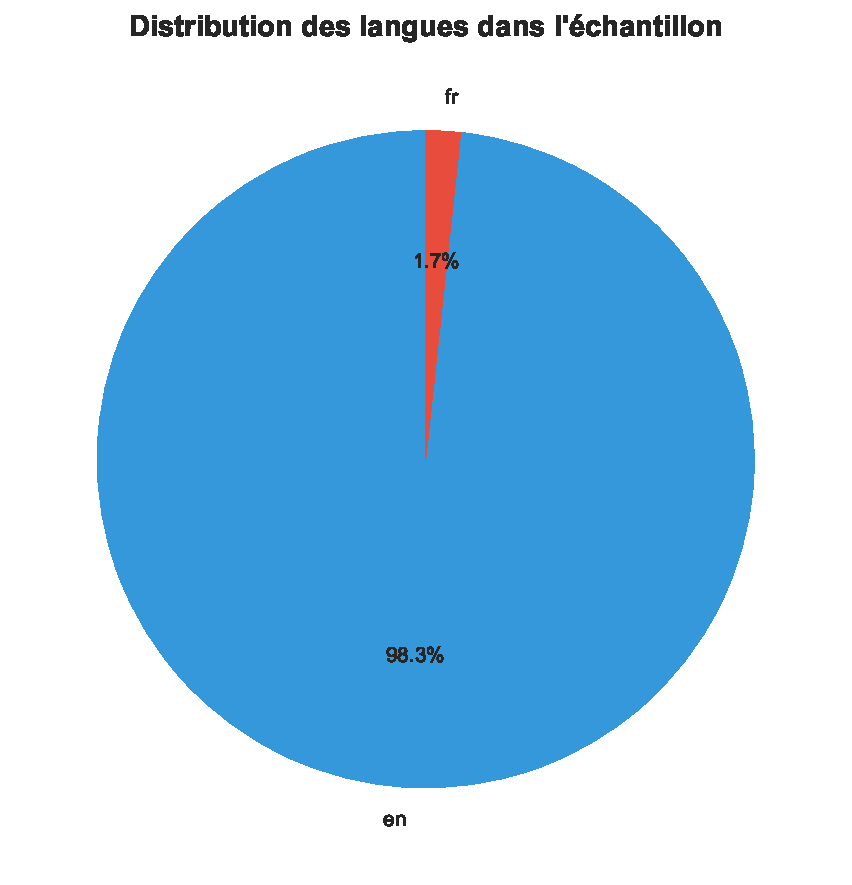
\includegraphics[width=0.75\textwidth]{figures/12_distribution_langues.pdf}
    \caption{Distribution globale des langues dans l'échantillon}
    \label{fig:distribution_langues}
\end{figure}

\begin{figure}[H]
    \centering
    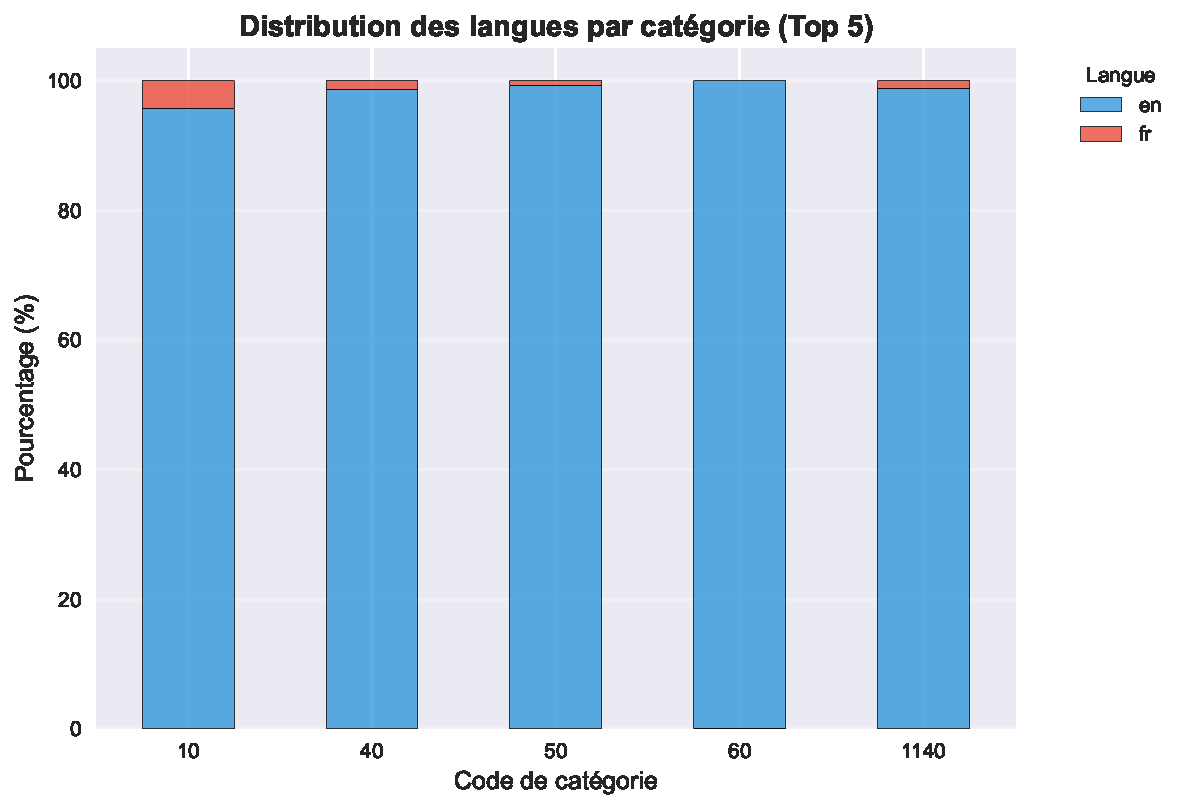
\includegraphics[width=0.9\textwidth]{figures/13_langues_par_categorie.pdf}
    \caption{Distribution des langues par catégorie (Top 5 catégories)}
    \label{fig:langues_par_categorie}
\end{figure}

\textbf{Observations :}
Les figures~\ref{fig:distribution_langues} et~\ref{fig:langues_par_categorie} montrent :
\begin{itemize}
    \item Le dataset est majoritairement multilingue, avec une prédominance de l'anglais (environ 98\%) et une présence du français (environ 2\%)
    \item Possible présence d'autres langues selon les catégories de produits
    \item Variation possible selon les catégories de produits
\end{itemize}

\textbf{Interprétation :}
La détection de langue peut être utile pour :
\begin{itemize}
    \item Adapter le prétraitement (stop words, stemming selon la langue)
    \item Identifier des patterns spécifiques à certaines langues
    \item Gérer les cas multilingues si présents
\end{itemize}

\subsection{Analyse des features additionnelles}

\subsubsection{Richesse du vocabulaire}

Deux visualisations principales :
\begin{enumerate}
    \item \textbf{Histogramme de la richesse du vocabulaire} : Distribution de la métrique (mots uniques / mots totaux)
    \item \textbf{Boxplot par catégorie (Top 10)} : Variation de la richesse selon la catégorie
\end{enumerate}

\begin{figure}[H]
    \centering
    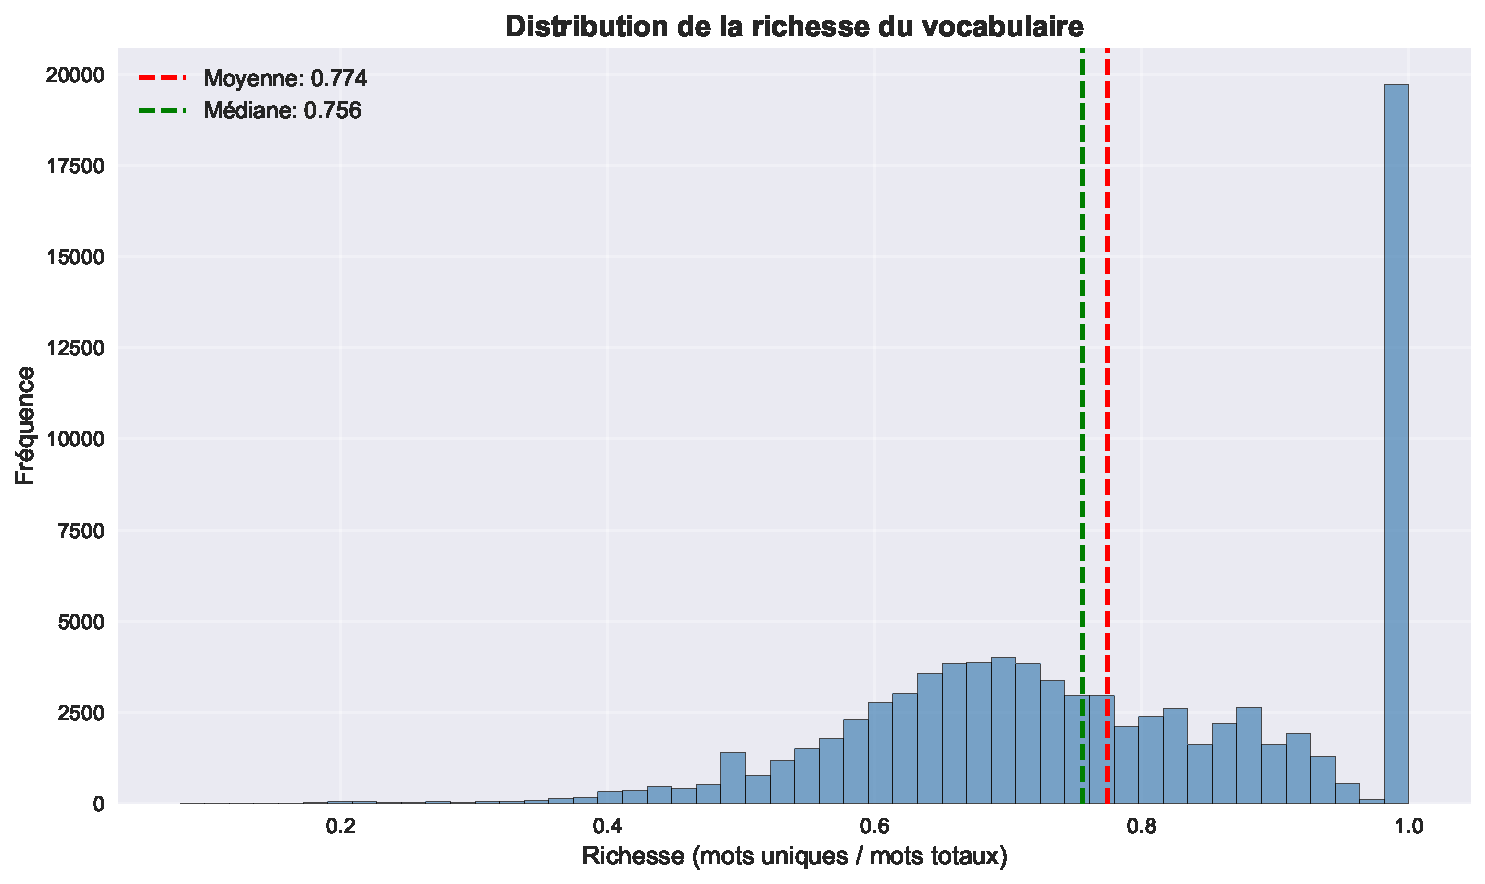
\includegraphics[width=0.85\textwidth]{figures/14_richesse_vocabulaire.pdf}
    \caption{Distribution de la richesse du vocabulaire (mots uniques / mots totaux)}
    \label{fig:richesse_vocabulaire}
\end{figure}

\begin{figure}[H]
    \centering
    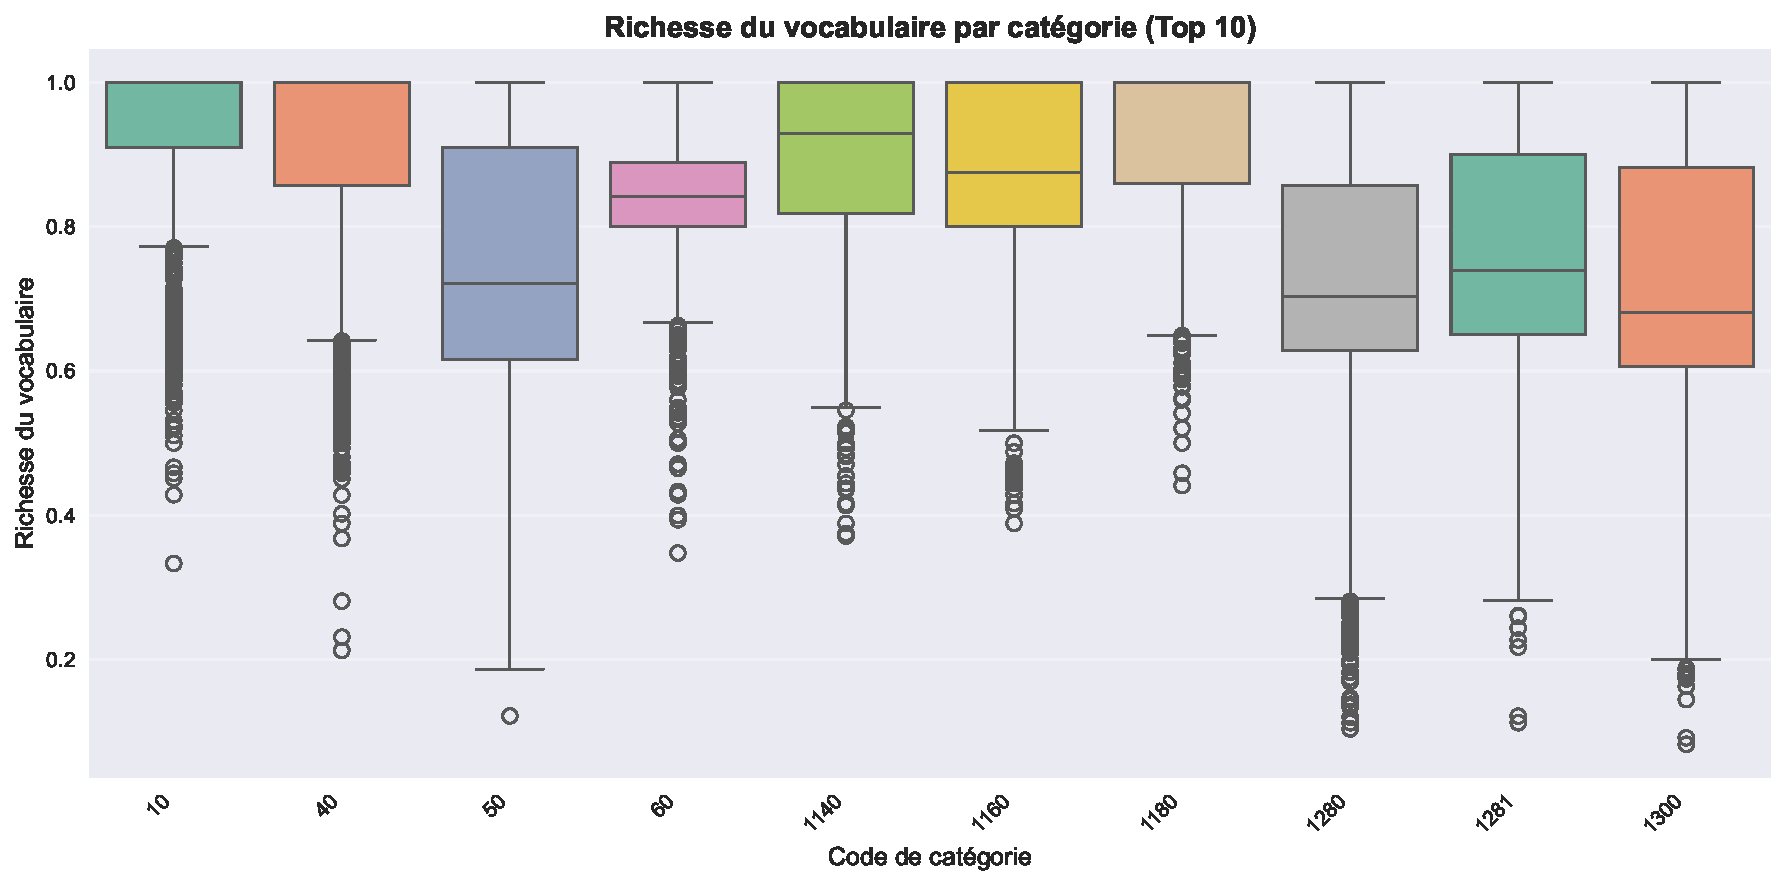
\includegraphics[width=0.9\textwidth]{figures/15_richesse_vocab_par_categorie.pdf}
    \caption{Richesse du vocabulaire par catégorie (Top 10)}
    \label{fig:richesse_vocab_par_categorie}
\end{figure}

\textbf{Observations :}
Les figures~\ref{fig:richesse_vocabulaire} et~\ref{fig:richesse_vocab_par_categorie} montrent :
\begin{itemize}
    \item La richesse du vocabulaire varie selon la catégorie
    \item Certaines catégories ont un vocabulaire plus diversifié que d'autres
    \item Distribution centrée autour de 0.75-0.80 (75-80\% de mots uniques)
    \item Variation significative entre les catégories (visible dans le boxplot)
\end{itemize}

\textbf{Interprétation :}
La richesse du vocabulaire est une feature discriminante potentielle. Les catégories avec un vocabulaire plus spécialisé (richesse plus élevée) peuvent être mieux différenciées. La relation avec la longueur suggère que les textes plus longs tendent à répéter plus de mots, réduisant la richesse.

\section{Nettoyage et prétraitement}

\textbf{Note sur le périmètre :} Concernant les données images (colonne \texttt{imageid}), une analyse préliminaire a montré qu'aucun nettoyage n'était nécessaire. Les images sont déjà correctement annotées et structurées. Par conséquent, ce rapport se concentre exclusivement sur le nettoyage et le prétraitement des données textuelles (\texttt{designation} et \texttt{description}).

\subsection{Nettoyage de base}

\subsubsection{Fonctions de nettoyage appliquées}

Une fonction \texttt{nettoyer\_texte()} a été implémentée avec les étapes suivantes :

\begin{enumerate}
    \item \textbf{Suppression des balises HTML}
    \begin{itemize}
        \item Expression régulière : \verb|r'<[^>]+>'|
        \begin{itemize}
            \item Le caractère \texttt{\textasciicircum} dans les crochets signifie "tout sauf"
        \end{itemize}
        \item Supprime toutes les balises HTML présentes dans les textes
    \end{itemize}
    
    \item \textbf{Remplacement des entités HTML}
    \begin{itemize}
        \item \texttt{\&nbsp;} $\rightarrow$ espace
        \item \texttt{\&amp;} $\rightarrow$ \&
        \item \texttt{\&lt;}, \texttt{\&gt;} $\rightarrow$ $<$, $>$
        \item \texttt{\&quot;} $\rightarrow$ "
        \item \texttt{\&\#39;} $\rightarrow$ '
        \item Caractères accentués : \texttt{\&eacute;}, \texttt{\&egrave;}, \texttt{\&ecirc;}, \texttt{\&agrave;}, etc.
    \end{itemize}
    
    \item \textbf{Normalisation des espaces}
    \begin{itemize}
        \item Remplacement des espaces multiples par un seul espace
        \item Suppression des espaces en début et fin de texte
    \end{itemize}
\end{enumerate}

\subsubsection{Résultats du nettoyage}

\begin{table}[H]
\centering
\begin{tabular}{@{}lrr@{}}
\toprule
\textbf{Type} & \textbf{Modifiées} & \textbf{Pourcentage} \\
\midrule
Designations & 4,313 & 5.08\% \\
Descriptions & 71~635 & 84,36~\% \\
\bottomrule
\end{tabular}
\caption{Statistiques du nettoyage}
\label{tab:stats_nettoyage}
\end{table}

\textbf{Exemples de modifications :}

\begin{itemize}
    \item \textbf{Suppression de balises HTML} : \texttt{$<$p$>$Texte$<$/p$>$} $\rightarrow$ \texttt{Texte}
    \item \textbf{Normalisation entités} : \texttt{\&eacute;l\&eacute;phant} $\rightarrow$ \texttt{éléphant}
    \item \textbf{Espaces multiples} : \texttt{Mot    mot} $\rightarrow$ \texttt{Mot mot}
    \item \textbf{Exemple réel} : 
    \begin{itemize}
        \item Avant : \texttt{Faber-Castell Lot De 3 Crayons ... À L\&\#39;Huile}
        \item Après : \texttt{Faber-Castell Lot De 3 Crayons ... À L'Huile}
    \end{itemize}
\end{itemize}

\subsection{Prétraitement avancé}

\subsubsection{Approche de prétraitement}

Le prétraitement avancé a été réalisé en utilisant la bibliothèque NLTK (Natural Language Toolkit) pour les opérations de traitement du langage naturel :

\begin{itemize}
    \item \textbf{Tokenisation} : Utilisation de \texttt{word\_tokenize} de NLTK pour une segmentation précise des mots
    \item \textbf{Suppression des stop words} : Élimination des mots vides français et anglais à partir des corpus NLTK
    \item \textbf{Stemming} : Réduction des mots à leur racine à l'aide de \texttt{SnowballStemmer} pour le français et l'anglais
\end{itemize}

\subsubsection{Fonction de prétraitement avancé}

La fonction \texttt{preprocess\_texte\_avance()} a été implémentée avec les paramètres suivants :

\begin{itemize}
    \item \texttt{remove\_stopwords=True} : Supprime les mots vides
    \item \texttt{stem=True} : Applique le stemming pour réduire les mots à leur racine
\end{itemize}

\textbf{Étapes du prétraitement :}
\begin{enumerate}
    \item Conversion en minuscules
    \item Suppression des caractères spéciaux (conservation des lettres, chiffres et espaces)
    \item Tokenisation avec NLTK
    \item Suppression des stop words français et anglais
    \item Stemming des tokens
    \item Reconstitution du texte à partir des tokens traités
\end{enumerate}

\textbf{Exemple :}
\begin{itemize}
    \item Avant : \texttt{"Belle chaise en bois massif pour salon"}
    \item Après (avec stop words et stemming) : \texttt{"bell chais bois massif salon"}
\end{itemize}

\subsection{Colonnes créées}

Après nettoyage et prétraitement, les colonnes suivantes ont été créées :

\begin{itemize}
    \item \texttt{designation\_clean} : Designation après nettoyage de base
    \item \texttt{description\_clean} : Description après nettoyage de base
    \item \texttt{texte\_complet} : Fusion de \texttt{designation\_clean} + \texttt{description\_clean}
\end{itemize}

\section{Features additionnelles}

\subsection{Features de longueur}

Ces features capturent la quantité d'information textuelle disponible :

\begin{table}[H]
\centering
\begin{tabular}{@{}lp{10cm}@{}}
\toprule
\textbf{Feature} & \textbf{Description} \\
\midrule
\texttt{len\_designation} & Nombre de caractères dans la designation \\
\texttt{len\_description} & Nombre de caractères dans la description \\
\texttt{len\_texte\_complet} & Nombre de caractères dans le texte complet \\
\texttt{nb\_mots\_designation} & Nombre de mots dans la designation \\
\texttt{nb\_mots\_description} & Nombre de mots dans la description \\
\texttt{nb\_mots\_total} & Nombre total de mots \\
\bottomrule
\end{tabular}
\caption{Features de longueur créées}
\label{tab:features_longueur}
\end{table}

\subsection{Features binaires}

\begin{table}[H]
\centering
\begin{tabular}{@{}lp{10cm}@{}}
\toprule
\textbf{Feature} & \textbf{Description} \\
\midrule
\texttt{has\_description} & 1 si description non vide, 0 sinon \\
\bottomrule
\end{tabular}
\caption{Features binaires créées}
\label{tab:features_binaires}
\end{table}

\subsection{Features de qualité textuelle}

\begin{table}[H]
\centering
\begin{tabular}{@{}lp{10cm}@{}}
\toprule
\textbf{Feature} & \textbf{Description} \\
\midrule
\texttt{richesse\_vocab} & Nombre de mots uniques / nombre total de mots \\
\texttt{moyenne\_longueur\_mots} & Longueur moyenne des mots en caractères \\
\texttt{nb\_caracteres\_speciaux} & Nombre de caractères spéciaux \\
\bottomrule
\end{tabular}
\caption{Features de qualité textuelle créées}
\label{tab:features_qualite}
\end{table}

\subsection{Statistiques des features créées}

\textbf{Features de longueur :}
\begin{itemize}
    \item Distributions similaires aux distributions des textes bruts
    \item Corrélations attendues entre longueurs de designation et description
\end{itemize}

\textbf{Features de qualité :}
\begin{itemize}
    \item \texttt{richesse\_vocab} : Varie selon la catégorie (certaines catégories ont un vocabulaire plus riche)
    \item \texttt{has\_description} : ~30\% des produits ont une description
    \item \texttt{moyenne\_longueur\_mots} : Peut identifier des patterns spécifiques (mots techniques longs vs mots courts)
\end{itemize}

\subsection{Dataset final préparé}

Le dataset final contient :

\textbf{Colonnes de base :}
\begin{itemize}
    \item \texttt{productid}, \texttt{imageid}
    \item \texttt{designation\_clean}, \texttt{description\_clean}, \texttt{texte\_complet}
    \item \texttt{prdtypecode} (variable cible)
\end{itemize}

\textbf{Features numériques :}
\begin{itemize}
    \item 10 features additionnelles créées
    \item Prêtes pour l'étape de modélisation
\end{itemize}

Ces observations préliminaires nous amènent à analyser plus en détail la distribution statistique des catégories.

\section{Conclusion}

Cette exploration approfondie du dataset Rakuten a permis d'identifier les caractéristiques principales des données textuelles et de préparer le terrain pour la phase de modélisation. Les analyses réalisées ont mis en évidence la structure du dataset, les défis à relever (déséquilibre des classes, descriptions manquantes, variabilité textuelle) et les opportunités offertes par les features additionnelles créées.

Le travail de nettoyage et de prétraitement effectué, ainsi que les visualisations développées, constituent une base solide pour orienter les choix d'architecture et de prétraitement lors de la phase de modélisation. Les insights obtenus permettront de développer des modèles de classification performants et adaptés aux spécificités de ce dataset.

\end{document}

